\documentclass[11pt,a4paper]{article}
% ===== Packages =====
\usepackage[utf8]{inputenc}
\usepackage[T1]{fontenc}
\usepackage{times}      % Times text; math in Computer Modern
\renewcommand{\ttdefault}{cmtt}
\usepackage{microtype}
\usepackage{amsmath,amssymb,amsthm}
\usepackage{booktabs}
\usepackage{array}
\usepackage{graphicx}
\usepackage{xcolor}
\usepackage{tikz}
\usetikzlibrary{arrows.meta,positioning}
\usepackage{geometry}
\usepackage[colorlinks=true,linkcolor=blue!50!black,citecolor=green!35!black,urlcolor=blue!50!black]{hyperref}
\geometry{a4paper,left=2.5cm,right=2.5cm,top=2.4cm,bottom=2.6cm}
\setlength{\parindent}{1.2em}
\setlength{\parskip}{0pt}
\setlength{\emergencystretch}{2em}
\renewcommand{\baselinestretch}{1.05}

% ----- Algorithm environments -----
\newcounter{alg}
\newenvironment{algorithm}[1][]{%
  \par\medskip\noindent\begin{minipage}{\linewidth}\hrule\vspace{3pt}%
  \renewcommand{\caption}[1]{\refstepcounter{alg}\textbf{Algorithm~\thealg.} ##1\par\vspace{3pt}\hrule\vspace{2pt}}}%
  {\vspace{2pt}\hrule\end{minipage}\par\medskip}
\newenvironment{algorithmic}{%
  \begin{list}{\small\arabic{enumi}:}{\usecounter{enumi}\setlength{\topsep}{2pt}\setlength{\itemsep}{1pt}%
  \setlength{\leftmargin}{2.2em}\setlength{\labelwidth}{1.6em}}}{\end{list}}
\newcommand{\State}{\item}
\newcommand{\For}[1]{\item \textbf{for} #1 \textbf{do}}
\newcommand{\EndFor}{\item \textbf{end for}}
\newcommand{\Comment}[1]{\hfill{\small$\triangleright$ #1}}
\newcommand{\Return}{\textbf{return}\ }

% ----- Headings, abstract and captions -----
\makeatletter
\renewcommand\@seccntformat[1]{\csname the#1\endcsname.\hspace{0.6em}}
\renewcommand\thesection{\Roman{section}}
\renewcommand\thesubsection{\Alph{subsection}}
% A reference to a subsection names its section too ("Sec. IV.B", not "Sec. B").
\renewcommand\p@subsection{\thesection.}
\renewcommand\thesubsubsection{\arabic{subsubsection}}
\renewcommand\p@subsubsection{\thesection.\thesubsection.}
\renewcommand\section{\@startsection{section}{1}{\z@}%
  {3.0ex \@plus 1ex \@minus .2ex}{1.4ex \@plus .2ex}%
  {\centering\normalfont\normalsize\bfseries}}
\renewcommand\subsection{\@startsection{subsection}{2}{\z@}%
  {2.2ex \@plus 1ex \@minus .2ex}{1.1ex \@plus .2ex}%
  {\centering\normalfont\small\bfseries}}
\renewcommand\subsubsection{\@startsection{subsubsection}{3}{\z@}%
  {1.8ex \@plus 1ex \@minus .2ex}{0.9ex \@plus .2ex}%
  {\centering\normalfont\small\bfseries\itshape}}
\renewcommand\paragraph{\@startsection{paragraph}{4}{\z@}%
  {1.6ex \@plus 1ex \@minus .2ex}{-0.6em}%
  {\normalfont\normalsize\itshape}}
\renewenvironment{abstract}{%
  \begin{quote}\small\noindent}{\end{quote}\vspace{0.6ex}}
\renewcommand\maketitle{\begin{center}%
  {\large\bfseries\@title\par}\vspace{1.4ex}%
  {\normalsize\@author\par}\vspace{0.4ex}%
  {\small\itshape\@date\par}\end{center}\vspace{0.6ex}}
\renewcommand*\l@section{\@dottedtocline{1}{0pt}{2.4em}}
\long\def\@makecaption#1#2{\vskip 6pt{\small\textsc{#1.}~#2\par}}
\makeatother
\renewcommand{\figurename}{Fig.}
\renewcommand{\refname}{References}
\numberwithin{equation}{section}
\renewcommand{\theequation}{\arabic{section}.\arabic{equation}}

% ----- Statements -----
\theoremstyle{plain}
\newtheorem{proposition}{Proposition}
\theoremstyle{remark}
\newtheorem{remark}{Remark}
% Marker for statements that are derived here but not checked independently

% ===== Notation =====
\newcommand{\dg}{^{\dagger}}
\newcommand{\Dpv}{D_{\mathrm{PV}}}
\newcommand{\Cpv}{C_{\mathrm{PV}}}
\newcommand{\Spv}{S_{\mathrm{PV}}}
\newcommand{\Bpv}{B_{\mathrm{PV}}}
\newcommand{\Pp}{P_{+}}
\newcommand{\Pm}{P_{-}}
\newcommand{\Gfive}{\Gamma_5}
\newcommand{\AR}{\tilde A_{R}}
\newcommand{\AL}{\tilde A_{L}}
\newcommand{\Pro}{\mathcal P}
\newcommand{\Dc}{\mathcal D_{\mathrm c}}
\newcommand{\Dcpv}{\mathcal D_{\mathrm c}^{\mathrm{PV}}}
\newcommand{\Hc}{\mathcal H_{\mathrm c}}
\renewcommand{\Re}{\operatorname{Re}}
\newcommand{\Ce}{C_{e}}
\newcommand{\Co}{C_{o}}
\newcommand{\Cpve}{C_{\mathrm{PV},e}}
\newcommand{\Cpvo}{C_{\mathrm{PV},o}}

% Implementation and numerical-results sections; off = theory-only note.
\newif\ifresults
\resultstrue

\title{Multigrid for the even-odd preconditioned M\"obius domain-wall operator\\
with a factorized Pauli--Villars coarse correction}
\author{Wei-Lun Chen\\[0.3ex]{\small\itshape draft}}
\date{\today}

\begin{document}
\maketitle

\begin{abstract}
Domain-wall fermions keep chiral symmetry up to effects that vanish as $L_s$ grows, but the cost
of inverting the M\"obius domain-wall operator rises steeply toward the physical light-quark mass,
because its spectrum surrounds the origin. Preconditioning with the Pauli--Villars operator moves
all eigenvalues into the right half-plane. We construct a two-grid method for this preconditioned
operator in which the quark and Pauli--Villars factors are coarsened separately. The outer system
is the even-odd one, every aggregate contains the whole fifth dimension so that the coarse lattice
is four-dimensional with nearest-neighbor couplings, and levels below the coarse lattice replace
deflation. These choices address the three reasons Boyle and Yamaguchi gave for why this approach
did not beat red-black CG. One setup serves every value of Neff's $\alpha$ and the solves with
$D\dg$ in HMC, for which $\Gfive D^{-1}\Gfive$ is a good preconditioner.\ifresults{} The field of
values of the preconditioned operator reaches into the left half-plane, yet its spectrum has
$\Re\lambda\ge0.78$, and its pseudospectra account for the convergence. On a quenched
$24^3\times48$ lattice the iteration count grows by a factor of $2$--$4$ from $m=0.1$ to
$m=0.001$, against $20$ for even-odd CGNE. At $m=0.001$ a solve is $4.5$--$4.8$ times faster than
mixed-precision CGNE, and a point-source propagator takes half its time, setup included. These
results come from one configuration per volume and a comparison with CGNE only.\else{} We state
the method and the questions that are open.\fi
\end{abstract}

\vspace{1ex}
{\small\noindent This paper is licensed under CC BY 4.0
(\url{https://creativecommons.org/licenses/by/4.0/}), except Figs.~\ref{fig:free}--\ref{fig:A},
reproduced from Ref.~\cite{KCM2024} under its CC BY-NC-ND 4.0.\par}
\vspace{1ex}

% ============================================================
\section{Introduction}
\label{sec:intro}

Many lattice computations need fermions whose chiral symmetry is broken only slightly at finite
lattice spacing. Weak matrix elements benefit from it, since operators of different chirality then
do not mix, as in the Standard Model calculation of $K\to\pi\pi$ decays and
$\varepsilon'/\varepsilon$~\cite{RBCKpipi}. It is used as well in precision calculations at the
physical quark masses: the hadronic vacuum polarization and light-by-light contributions to the
muon $g-2$~\cite{RBCHVP,RBCWindow,RBCHLbL}, the $B\to\pi\ell\nu$ form factors on fine lattices
with the heavy quark in the same M\"obius domain-wall action~\cite{JLQCDBpi}, and inclusive
semileptonic $B$ decays~\cite{HashimotoInclusive,GambinoInclusive,BaroneInclusive}. The overlap operator~\cite{NarayananNeuberger,Neuberger} has an exact lattice
chiral symmetry. Domain-wall fermions~\cite{Kaplan,Shamir,FurmanShamir} approximate it at a lower
cost. They add a fifth dimension of extent $L_s$, and a large negative Wilson mass $-M_5$ binds
modes of opposite chirality to its two boundaries. The residual breaking of chiral symmetry falls
as $L_s$ grows. The M\"obius generalization~\cite{BNO0,BNO1,BNO} adds two coefficients $(b,c)$
and improves the approximation at fixed $L_s$; $c=0$ is Shamir's operator.

Solving with the domain-wall operator is expensive, because it is neither Hermitian nor positive and one application costs $L_s$ four-dimensional Wilson hops. The standard solver is
still the conjugate gradient method on the normal equation of the even-odd operator (CGNE),
whose condition number is the square of that of the operator. For Wilson fermions, multigrid
solved this problem. The low modes that slow down Krylov solvers are locally
coherent~\cite{Luscher}: a few of them, cut into blocks, span the low-mode space. Adaptive
aggregation multigrid uses this, and its cost hardly depends on the quark
mass~\cite{Brannick,DDalphaAMG,BridgeMG}.

\paragraph{Multigrid for domain-wall fermions.}
For domain-wall fermions multigrid is harder. Because of the large negative Wilson mass, the
spectrum encloses the origin. Non-Hermitian Krylov methods then converge only after a number of
steps of the order of the system size~\cite{NRT,BoyleMRHS}. Boyle~\cite{BoyleMRHS} lists four
approaches that work to some extent. They differ in the operator that is coarsened.
\begin{itemize}
\item Cohen \textit{et al.}~\cite{Cohen} coarsened the squared operator, with blocks that cover
the whole fifth dimension. Its coarse operator reaches two hops.
\item HDCG~\cite{HDCG} accelerates CGNE and coarsens the squared even-odd Schur complement. Its
coarse stencil has $81$ points for blocks of at least $4^4$.
\item HDCR~\cite{HDCR} coarsens the Hermitian indefinite operator $\gamma_5RD$ at $c=0$. Its
coarse operator stays nearest-neighbor, which keeps the setup affordable in HMC.
\item Brower, Clark, Howarth and Weinberg~\cite{BCHW} noted that the Pauli--Villars preconditioned
operator $\Dpv^{-1}D$ carries the physical four-dimensional degrees of freedom. They solved
$\Dpv\dg Dx=\Dpv\dg b$ on the whole lattice. Projecting the Wilson kernel slice by slice gives
coarse operators $\hat D$ and $\hat D_{\rm PV}$, both nearest-neighbor, and the coarse correction
solves $\hat D_{\rm PV}\dg\hat D\,\hat e=\hat r$. They tested Shamir fermions in the
two-dimensional Schwinger model.
\end{itemize}
Boyle and Yamaguchi~\cite{BY} compared these approaches for Shamir fermions and found that on large volumes HDCR was set up and solved faster than a single even-odd CG solve. They also carried the
Pauli--Villars method of Ref.~\cite{BCHW} to four-dimensional QCD. On a $16^3\times32$
Shamir configuration at $m=0.001$ it needed about half the fine-matrix applications of red-black
CG, but a solve took $1089$--$1904$\,s against $62$\,s (one right-hand side, setup excluded,
double precision), and they named three
reasons. The method works on the whole lattice, while red-black CG is the relevant baseline. Its
coarse space keeps a fifth dimension of extent $L_s$, which makes the coarse solves costly. And its coarse solves are non-Hermitian and were not deflated, while the non-normal case would need the
pseudospectrum and a singular value decomposition. Two further findings matter here.
First, CG on the Schur complement $M_{ee}-M_{eo}M_{oo}^{-1}M_{oe}$ needed far fewer iterations
than on the left-preconditioned $1-M_{ee}^{-1}M_{eo}M_{oo}^{-1}M_{oe}$. Second, an even-odd
smoother did not work with the HDCR correction, which they traced to eigenvectors that are not aligned.

\paragraph{Recent work by Boyle and collaborators.}
The multiple right-hand-side HDCG of Ref.~\cite{BoyleMRHS} solves the normal equation of the
even-odd operator with a two-level conjugate gradient. Its coarse space is spanned by blocked
low modes from Chebyshev filters. Treating many right-hand sides at once makes the coarse space
cheap, and gains of up to twenty over even-odd CG are reported at physical quark mass. In a
Lattice~2026 talk, Boyle and Oare~\cite{BoyleOare} named two limits of this approach: forming the
$81$-point coarse operator is expensive, and a single solve on a new gauge field, as in HMC,
gains nothing from many right-hand sides. They coarsen the two-hop operator $\Dpv\dg D$ instead,
which gives a $33$-point stencil. They stressed that $\Dpv\dg D$ is non-normal: its field of
values can reach the left half-plane although its spectrum does not, so the GCR bound of
Eisenstat, Elman and Schultz~\cite{ESS} is lost. They added a shift to the smoothers. On a
$48^3\times96$ lattice at the physical quark mass they reported $578$ fine-matrix applications,
against $1100$ for HDCG and $26500$ for red-black CG. The coarse solve took $90\%$ of the time,
and they named the missing Lanczos deflation of the coarse operator as its limit.

\paragraph{Setup cost in ensemble generation.}
A multigrid setup is paid once per gauge field. This is affordable for propagators but not for
HMC, where the field changes at every step. Eick and Mawhinney~\cite{EickMawhinney} avoid the
setup by renormalization-group blocking: a fine M\"obius ensemble is blocked to a coarse lattice
whose domain-wall operator approximates the low modes of the fine one. They find that the
interpolated correction carries high modes that the fine operator amplifies by four orders of
magnitude, and they need a Chebyshev low-pass filter of degree $150$--$300$.

\paragraph{The preconditioned operator.}
Kanamori, Chen and Matsufuru~\cite{KCM2024} examined the spectra of several preconditioned
M\"obius operators. The operator $A'=(\Dpv\Cpv^{-1})\dg DC^{-1}$, which combines the
Pauli--Villars factor with the site-diagonal part $C$, has all eigenvalues in the right
half-plane and the smallest condition number among those they studied. With $\Dpv$ truncated to
blocks, negative real parts come back. Separately, Neff's form of the domain-wall
matrix~\cite{Neff,CKMN} rescales the fifth dimension by a site-local factor $Q$ and changes the
conditioning of the even-odd system.

\paragraph{This paper.}
We construct a two-grid method for $A'$ that takes up the Pauli--Villars route of
Refs.~\cite{BCHW,BY} and addresses the three reasons of Ref.~\cite{BY} in turn. It is an
adaptive aggregation multigrid in the sense
of Refs.~\cite{Brannick,DDalphaAMG,BridgeMG}: the coarse space comes from computed near-null vectors
cut into aggregates, and the coarse operators are Galerkin projections. First, the outer system is
the even-odd one, as for red-black CG. Its inverse contains the inverses of the quark operator and the
adjoint Pauli--Villars operator, with site-local factors and the restriction to the even sites
between them, and we replace each inverse by a Galerkin inverse, as Ref.~\cite{BCHW} does on the
whole lattice. Second, every aggregate contains the whole fifth dimension, so the coarse lattice is
four-dimensional and both coarse operators are nearest-neighbor. Third, the Pauli--Villars coarse
system is solved in a $\Sigma$-Hermitian form by MINRES, and levels below the coarse lattice with
a dense LU at the bottom take the place of deflation (Sec.~\ref{sec:coarse}). The test vectors are approximate right singular vectors of the
non-normal operator. The prolongation lifts these vectors to the whole lattice in
two ways, one for each coarse solve; for the right form this makes the correction exact on them
(Proposition~\ref{prop:exact}).\ifresults{} The left form used in practice is not exact, but
with the same vectors $y$ it still needs $\hat t$ (Sec.~\ref{sec:basischoice}).\fi The smoother is a fixed
Chebyshev polynomial, and the setup combines Chebyshev filtering with a bootstrap. For HMC we
also solve with $D\dg$. We show that the multigrid of $D$, placed between two $\Gfive$, is a good
preconditioner for $D\dg$, with no second setup.\ifresults{} We give numerical results: the
field of values, spectrum and pseudospectra of the preconditioned operator, the behavior of
truncated GCR, a mass scan and point-source propagators against CGNE, the sensitivity to the
parameters, and the solves with $D\dg$. All of it is on one GPU, and a comparison with HDCG and with
the coarsening of $\Dpv\dg D$ in one implementation is left open.\fi

Section~\ref{sec:overview} describes the method in words. Section~\ref{sec:opsec} recalls the
spectra the construction rests on and defines the operator, its preconditioning and the even-odd
forms. Section~\ref{sec:method} gives the two-grid method: the factorized correction, the coarse
solvers, the setup, the smoother and the outer solver. Section~\ref{sec:dagger} solves with
$D\dg$.\ifresults{} Section~\ref{sec:results} gives the results: first the cost against CGNE, with $D\dg$ and
in HMC, then what each part of the method contributes, then why it converges. Section~\ref{sec:summary} sums up.\fi{} Section~\ref{sec:open}
lists open problems. Appendix~\ref{sec:notation}
relates our notation to other references\ifresults{}, Appendix~\ref{sec:configs} lists the gauge
configurations\fi. The companion text
\texttt{docs/mg\_background/MG\_WALKTHROUGH.tex} in the RutticeQCD repository derives every
formula of this paper line by line.

\paragraph{Conventions.}
Five-dimensional fields are $\psi_s(x)$ with $s=0,\dots,L_s-1$, and $\Pp,\Pm=\tfrac12(1\pm\gamma_5)$.
$R$ reverses the fifth dimension, $(R\psi)_s=\psi_{L_s-1-s}$, and $\Gfive=\gamma_5R$. The subscripts
$e$ and $o$ denote blocks on the even and odd four-dimensional sites, and $X_{pq}$ maps parity $q$
to parity $p$. The injection $\iota$ puts a field on the even sites onto the whole lattice, with
zero on the odd sites, and $\pi=\iota\dg$ takes the even sites. Section~\ref{sec:operator} defines
the operator and its parts $C$ and $Q$.

% ============================================================
\subsection{Overview of the method}
\label{sec:overview}

This subsection describes the method in words, for readers who know domain-wall fermions but not
multigrid. The later sections give the equations.

\paragraph{Multigrid in one paragraph.} A multigrid preconditioner removes the error of an
iterate in two parts. The high modes are damped by a few steps of a cheap iteration on the fine
lattice, the \emph{smoother}. The low modes, the near-zero modes that make CG slow, are removed by
solving a much smaller problem on a \emph{coarse lattice}. The coarse lattice comes from
\emph{aggregation}. We cut the fine lattice into blocks of $4^4$ sites that contain the whole fifth
dimension. Each block becomes one coarse site, and its degrees of freedom are a few approximate low
modes restricted to the block, the \emph{test vectors}. The \emph{prolongation} $\Pro$ maps a
coarse vector to the fine lattice through these vectors, and $\Pro\dg$ maps back. The coarse
operator of a fine operator $X$ is its \emph{Galerkin} projection $\Pro\dg X\Pro$; it couples only
neighboring coarse sites if $X$ couples only neighboring fine sites. A few vectors per block
suffice because low modes are locally coherent~\cite{Luscher}. Finding the test vectors is the
\emph{setup}. It is paid once per gauge field and shared by all right-hand sides.

\paragraph{What is solved.} As in even-odd CGNE, we reduce $D\psi=\eta$ to the even sites, here
with the preconditioning of $A'$. This gives a system $\tilde Ay=\rho$, and we recover $\psi$
from $y$ afterwards. In practice $\tilde A$ is the left form $\AL$, which can carry Neff's
$\alpha$ (Sec.~\ref{sec:eo}). The outer solver is flexible GCR that keeps two directions, GCR(2).
Each of its iterations applies one two-grid cycle as the preconditioner (Sec.~\ref{sec:outer}).

\paragraph{One cycle.} A cycle is the smoother (a Chebyshev polynomial in $\tilde A$), a coarse
correction, and the smoother again (Algorithm~\ref{alg:cycle}). Coarsening $\tilde A$ itself would give a coarse stencil of $81$ points, because $\tilde A$
reaches four hops on the even sites. Instead we invert its two factors separately, as Ref.~\cite{BCHW} does on the whole lattice: first the
adjoint Pauli--Villars operator, then the quark operator. Each inverse is replaced by the Galerkin
inverse of $\Dpv$ or $D$, whose coarse stencil has $9$ points (Fig.~\ref{fig:correction},
Sec.~\ref{sec:correction}). Both coarse systems are solved only roughly, to a relative residual of
about $0.1$, in single precision and on the even coarse sites (Sec.~\ref{sec:coarse}).

\paragraph{The setup.} The setup has four steps (Algorithm~\ref{alg:setup}, Sec.~\ref{sec:setup}).
\begin{enumerate}
\item A Chebyshev filter applied to random vectors gives approximate low modes $y$ of $\AR$: the
vectors of its smallest singular values.
\item A bootstrap improves them. We build the cycle from the current vectors and apply a few
FGMRES steps with it to each vector; this enriches the vector in what the cycle still misses.
\item We lift each $y$ to the whole lattice in two ways, $s$ and $\hat t$, one for each coarse
solve. For the right form this makes the correction exact on these vectors
(Proposition~\ref{prop:exact}); the left form is not exact (Sec.~\ref{sec:basis}).
\item We split the lifts by their $\Gfive$-chirality and orthonormalize them on each block. This
gives $\Pro$, and from it the coarse operators of $D$ and $\Dpv$.
\end{enumerate}
All of the setup uses the plain $D$ and $\Dpv$. Neff's $\alpha$ enters only the outer operator
$\AL^{(\alpha)}$, the smoother, which works on it, and the site-local factors of the correction
(Eq.~\eqref{eq:corr}), so one setup serves both forms and every $\alpha$.

\paragraph{Solving with $D\dg$.} HMC also solves with $D\dg$. The same cycle, placed between two
$\Gfive$, is a good preconditioner for it (Sec.~\ref{sec:dagger}), so no second setup is needed.

\paragraph{Where to read on.} The construction is in Secs.~\ref{sec:eo} and \ref{sec:correction};
Table~\ref{tab:approaches} compares it with other multigrid methods for domain-wall
fermions.\ifresults{} The parameters used in practice are in Table~\ref{tab:setups}, and the
comparison with CGNE is in Sec.~\ref{sec:massscan}.\fi

% ============================================================
\section{The operator and its preconditioning}
\label{sec:opsec}

\subsection{Spectra of preconditioned M\"obius operators}
\label{sec:spectra}

Where the spectrum lies decides which iterative methods can work. A Krylov method builds a
residual polynomial $p$ with $p(0)=1$ that should be small on the spectrum. Such a polynomial of
low degree exists only if a region that excludes the origin, such as an ellipse, encloses the
spectrum. The Chebyshev smoother of Sec.~\ref{sec:smoother} needs the same, since it is defined by
an ellipse in the right half-plane. Both therefore need the eigenvalues on one side of the
origin. Those of the domain-wall operator do not, and the
preconditioners below move them there. Figures~\ref{fig:free}--\ref{fig:A}, from
Ref.~\cite{KCM2024}, show what each preconditioner does; the captions give the lattices.

\begin{figure}[tbp]
\centering
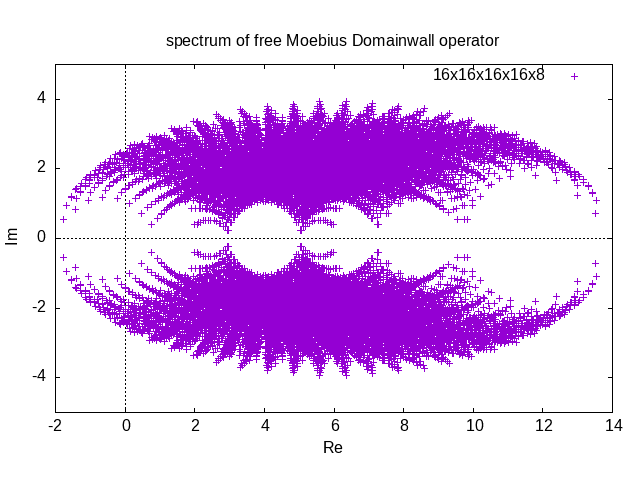
\includegraphics[width=0.6\linewidth]{spectrum_fig1.png}
\caption{Spectrum of a free M\"obius domain-wall operator on $16^4\times8$ with
quark mass $0.01$, $b=1.5$, $c=0.5$ and domain-wall height $M_5=1$.
Reproduced from Ref.~\cite{KCM2024}, Fig.~1, under its license CC BY-NC-ND 4.0.}
\label{fig:free}
\end{figure}

\paragraph{The unpreconditioned operator.}
The free spectrum (Fig.~\ref{fig:free}) is a band that reaches into $\Re\lambda<0$. On a
$2+1$-flavor configuration at the physical point (Fig.~\ref{fig:pv}, top left) the real parts
lie in $[-1.29,13.2]$. So CG and BiCGStab do not work on $D$ itself, and the practical choice has
been CG on a positive definite squared operator.

\paragraph{Site-diagonal preconditioning.}
The site-diagonal part $C$ has an inverse that is the same matrix on every site
(Sec.~\ref{sec:C}). With it, $DC^{-1}$ has real parts in $[-0.22,2.22]$ (middle left). The
spectrum shrinks, but it still lies on both sides of the origin.

\paragraph{Pauli--Villars preconditioning.}
The operator $\Dpv^{-1}D$, with $\Dpv=D(m=1)$, approximates the overlap operator~\cite{BCHW}.
Since $\Dpv^{-1}$ costs as much as a solve with $D$, Ref.~\cite{BCHW} used $\Dpv\dg$ instead.
$\Dpv\dg D$ has positive real parts (top right). Its low modes lie close to the imaginary axis,
shifted by about the quark mass, as for an overlap operator. Its high end, however, reaches about
$187$, which an overlap operator would not. If we replace $\Dpv$ by its block-diagonal
approximation $\Bpv$, which drops the hops between $4^4$ blocks, negative real parts come back
(middle and bottom right).

\paragraph{Both together.}
The operator $A'=(\Dpv\Cpv^{-1})\dg DC^{-1}$ has real parts in $[2.67\times10^{-4},\,5.22]$
(Fig.~\ref{fig:A}, left). Its condition number, $1.96\times10^{4}$, is smaller than the
$2.34\times10^{4}$ of $\Dpv\dg D$ and the smallest in Ref.~\cite{KCM2024}. With $\Dpv$ replaced
by $\Bpv$, the real parts become negative again (right). So a preconditioner that truncates the
Pauli--Villars factor to blocks would inherit eigenvalues with negative real part. Our method keeps
the factor exact on the fine lattice and approximates it only through its Galerkin coarse
operator (Sec.~\ref{sec:correction}).

\begin{figure}[tbp]
\centering
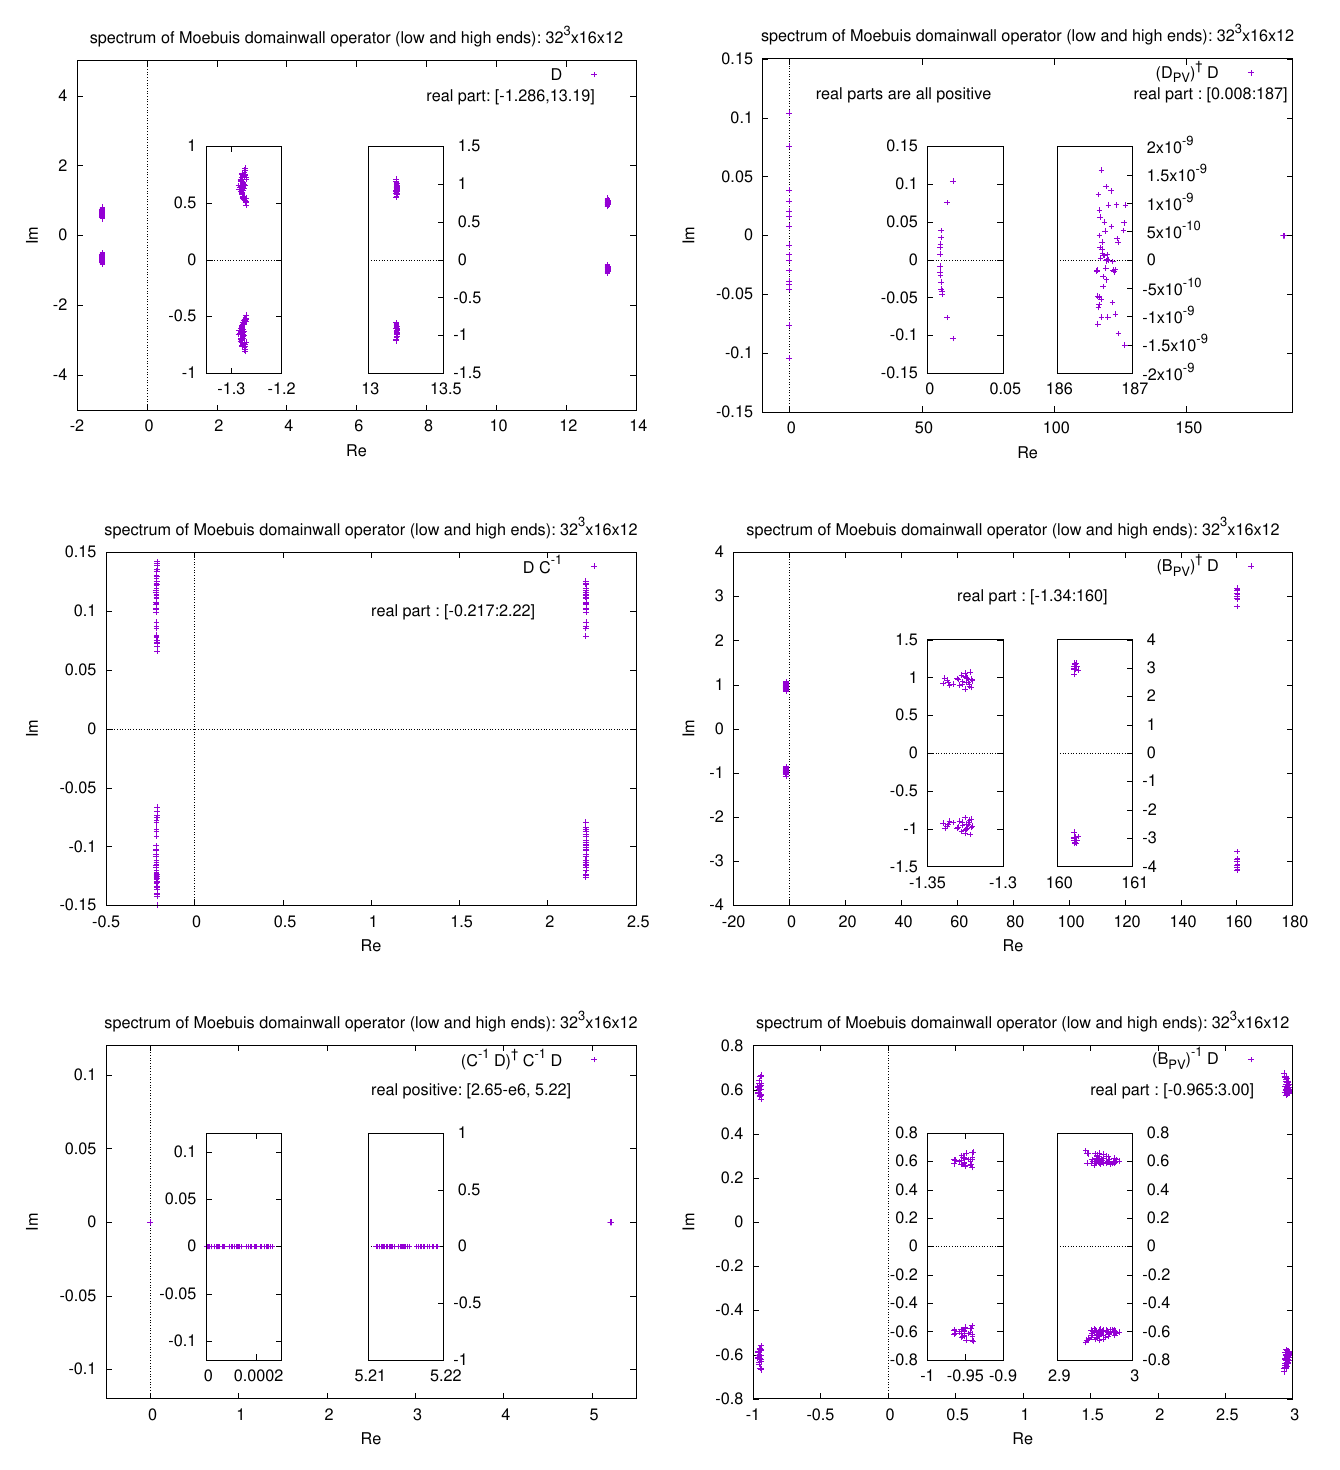
\includegraphics[width=\linewidth]{spectrum_fig3.png}
\caption{Low and high ends of the spectrum of the M\"obius operator on a
JLQCD $2+1$-flavor configuration at the physical point, with preconditioners.
Left column: $D$, $DC^{-1}$, $(C^{-1}D)\dg C^{-1}D$. Right column:
$\Dpv\dg D$, $\Bpv\dg D$, $\Bpv^{-1}D$, where $\Bpv$ is the block-diagonal
approximation of $\Dpv$ (inverted approximately in the last panel). The text of
Ref.~\cite{KCM2024} quotes $48^3\times16$ with $L_s=12$; the panel titles read
$32^3\times16\times12$. Reproduced from Ref.~\cite{KCM2024}, Fig.~3, under its license CC BY-NC-ND 4.0.}
\label{fig:pv}
\end{figure}

\begin{figure}[tbp]
\centering
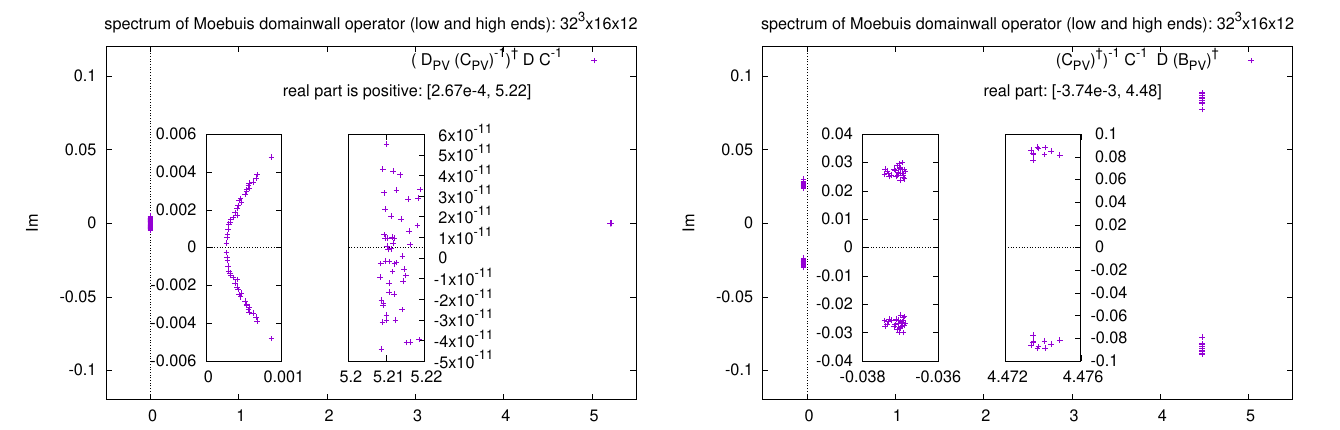
\includegraphics[width=\linewidth]{spectrum_fig4.png}
\caption{Left: spectrum of $A'=(\Dpv\Cpv^{-1})\dg DC^{-1}$, Eq.~\eqref{eq:Aprime},
on the configuration of Fig.~\ref{fig:pv}; all real parts are positive. Right:
the same with $\Dpv$ replaced by its block-diagonal approximation $\Bpv$; negative
real parts reappear. Lattice size as in Fig.~\ref{fig:pv} (the text of the source
quotes $48^3\times16$, $L_s=12$; the panel titles read $32^3\times16\times12$).
Reproduced from Ref.~\cite{KCM2024}, Fig.~4, under its license CC BY-NC-ND 4.0.}
\label{fig:A}
\end{figure}

\paragraph{Two caveats.}
First, the figures show the full-lattice operator $A'$, not the even-odd operators of
Sec.~\ref{sec:eo}. Second, positive real parts of the eigenvalues do not mean a positive field of
values. For a non-normal operator the GCR bound~\cite{ESS} needs the Hermitian part
$(A+A\dg)/2$ to be positive definite. This can fail while every eigenvalue lies in the right
half-plane, as Ref.~\cite{BoyleOare} discusses for $\Dpv\dg D$.
\ifresults{}It occurs for the even-odd form: for $\AR$ itself the field of values reaches just
below zero on $12^4$ ($\Re W\ge-4.6\times10^{-3}$ with stout smearing,
$-5.0\times10^{-2}$ without), and for the multigrid-preconditioned $\AR\mathcal M$ far
below (Sec.~\ref{sec:fov}). The bound of Ref.~\cite{ESS} is then lost, but the
spectrum of $\AR\mathcal M$ stays at $\Re\lambda\ge0.78$ and its pseudospectra bound
full GMRES (Secs.~\ref{sec:spectrum}, \ref{sec:pseudo}); truncated GCR is not covered
(Sec.~\ref{sec:gcrk}). For the full-lattice $A'$ it has not been measured.\else{}Whether
it occurs for $A'$ and its even-odd forms is open (Sec.~\ref{sec:open}).\fi

% ============================================================
\subsection{The operator and Pauli--Villars preconditioning}
\label{sec:operator}

This subsection defines the M\"obius operator in the form of Brower, Neff and
Orginos~\cite{BNO} and derives from it the quantities the method is built on: the
part $C$ of the operator that acts within a four-dimensional site and its inverse, the
$\Gfive$-transformation of $D$, the Pauli--Villars preconditioned operator $A'$ of
Ref.~\cite{KCM2024}, and Neff's $\alpha$. The notation
follows Ref.~\cite{BNO} except where stated; Appendix~\ref{sec:notation} relates it to
Ref.~\cite{KCM2024} and to Bridge++ symbol by symbol.

\subsubsection{The M\"obius operator}
\paragraph{Ingredients.} $\psi$ is a field on the four-dimensional lattice with an extra
index $s=0,\dots,L_s-1$, the fifth dimension; $\psi_s$ is an ordinary Dirac field for each
$s$. $P_\pm=\tfrac12(1\pm\gamma_5)$ are the chiral projectors. The Wilson hopping term is
\begin{equation}
(K\psi)(x)=\sum_{\mu=1}^{4}\Big[(1-\gamma_\mu)U_\mu(x)\psi(x+\hat\mu)
+(1+\gamma_\mu)U_\mu\dg(x-\hat\mu)\psi(x-\hat\mu)\Big],
\end{equation}
and the Wilson operator with mass $-M_5$ (the domain-wall height $M_5>0$) is
\begin{equation}
W=(4-M_5)-\tfrac12K .
\label{eq:W}
\end{equation}
This is the usual $D_W(-M_5)$ with hopping coefficient $\tfrac12$; in the $\kappa$
normalization $W=(4-M_5)(1-\kappa K)$ with $\kappa=1/(8-2M_5)$. $W$ acts on each slice
$s$ in the same way and does not mix slices. Its free spectrum, needed in
Sec.~\ref{sec:dagger}, is $\{-M_5+\sum_\mu(1-\cos p_\mu)\pm i(\sum_\mu\sin^2p_\mu)^{1/2}\}$.

\paragraph{The operator.} With
\begin{equation}
D_+=1+bW,\qquad D_-=cW-1
\label{eq:Dpm}
\end{equation}
(Ref.~\cite{BNO}, Eq.~(2.18)), the M\"obius operator at quark mass $m$ acts slice by slice as
\begin{equation}
(D\psi)_s=D_+\psi_s+D_-\big(\Pm\psi_{s+1}+\Pp\psi_{s-1}\big),\qquad
\psi_{L_s}\equiv-m\,\psi_0,\quad \psi_{-1}\equiv-m\,\psi_{L_s-1}
\label{eq:Dslice}
\end{equation}
(Ref.~\cite{BNO}, Eq.~(2.20), with $s$ counted from $0$). For $L_s=4$, as a matrix in $s$,
\begin{equation}
D=\begin{pmatrix}
D_+ & D_-\Pm & 0 & -mD_-\Pp\\
D_-\Pp & D_+ & D_-\Pm & 0\\
0 & D_-\Pp & D_+ & D_-\Pm\\
-mD_-\Pm & 0 & D_-\Pp & D_+
\end{pmatrix}.
\label{eq:Dmatrix}
\end{equation}
Shamir's operator is $b=1$, $c=0$; the results of this paper use $b=1.5$, $c=0.5$
($b-c=1$, $b+c=2$). The quark mass enters only through the two corners. The physical
four-dimensional quark field is $q=\Pm\psi_0+\Pp\psi_{L_s-1}$.

\paragraph{The hop in the fifth dimension.} Eq.~\eqref{eq:Dslice} separates into a part
that hops in the fifth dimension and one that does not. Define
\begin{equation}
(Y\psi)_s=-\Pm\psi_{s+1}-\Pp\psi_{s-1}\qquad\text{(with the same wrap-around)},
\label{eq:Y}
\end{equation}
the off-diagonal part of Eq.~\eqref{eq:Dmatrix} without $D_-$ and with a minus sign. Then
$D=D_+-D_-Y$. Here $D_-$ stands to the \emph{left} of $Y$, since in Eq.~\eqref{eq:Dslice} it
acts on the shifted and projected field, and this order matters in Sec.~\ref{sec:g5}. Inserting
Eqs.~\eqref{eq:W} and \eqref{eq:Dpm},
\begin{equation}
D=1+bW-(cW-1)Y=1+Y+W\,(b-cY)=C-\tfrac12K\,(b-cY),\qquad C=d_++d_-Y,
\label{eq:D}
\end{equation}
with $d_+=1+b(4-M_5)$ and $d_-=1-c(4-M_5)$. In the last step $W=(4-M_5)-\frac12K$ was split
into its site-local constant and its hop; the constant parts form $C$. Note
$d_-=-(c(4-M_5)-1)$ is \emph{minus} the site-local part of $D_-$, because $Y$ carries the
sign. The Pauli--Villars operator is the same operator at unit mass, $\Dpv=D|_{m=1}$,
$\Cpv=C|_{m=1}$; $D_\pm$ and $K$ do not depend on $m$.

\subsubsection{\texorpdfstring{$\Gfive$}{Gamma5}-transformation and the exact adjoint}
\label{sec:g5}
For the Wilson operator $\gamma_5W\gamma_5=W\dg$, so a solve with $W\dg$ is a solve with $W$
between two multiplications by $\gamma_5$. The analogue for domain-wall fermions uses
\begin{equation}
\Gfive=\gamma_5R,\qquad (R\psi)_s=\psi_{L_s-1-s} .
\end{equation}
Each building block transforms as follows.
\begin{enumerate}
\item $W$, $D_+$, $D_-$: they act on every slice alike, so they commute with $R$, and
$\gamma_5W\gamma_5=W\dg$. Hence $\Gfive W\Gfive=W\dg$, $\Gfive D_\pm\Gfive=D_\pm\dg$.
\item $Y$: it has no hop in the four dimensions, so $\Gfive Y\Gfive$ can be read off
Eq.~\eqref{eq:Y}. $\gamma_5$ commutes with $P_\pm$; $R$ turns the hop $s\to s+1$ into
$s\to s-1$. So $\Gfive Y\Gfive$ has $-\Pm$ on the hop down and $-\Pp$ on the hop up,
and the corner $-m$ moves to the other corner. This is the transpose of
Eq.~\eqref{eq:Y} in $s$ with $P_\pm$ in place, which is $Y\dg$ since $P_\pm\dg=P_\pm$ and $m$
is real: $\Gfive Y\Gfive=Y\dg$.
\item $W$ and $Y$ do not commute: $\gamma_\mu$ in $K$ anticommutes with $\gamma_5$, so
$\gamma_\mu P_\pm=P_\mp\gamma_\mu$, and the hop of $K$ exchanges the two projectors of $Y$.
\end{enumerate}
From $D=D_+-D_-Y$ it follows that
\begin{equation}
\Gfive D\Gfive=D_+\dg-D_-\dg Y\dg ,\qquad\text{whereas}\qquad D\dg=D_+\dg-Y\dg D_-\dg ,
\label{eq:g5D}
\end{equation}
the adjoint reversing the order of the product. The difference is a commutator,
\begin{equation}
\Gfive D\Gfive-D\dg=Y\dg D_-\dg-D_-\dg Y\dg=c\,[Y\dg,W\dg]=\tfrac{c}{2}\big[K\dg,Y\dg\big],
\label{eq:g5herm}
\end{equation}
where $D_-\dg=cW\dg-1$ and $W\dg=(4-M_5)-\frac12K\dg$ were used. It vanishes for Shamir's
operator ($c=0$) and is of order $c$ otherwise. Thus $\Gfive D\Gfive\neq D\dg$ for M\"obius
fermions: a multigrid built for $D$ cannot be used for $D\dg$ by conjugating with $\Gfive$.
\ifresults{} On a $12^4$ configuration with stout links ($M_5=1$, $m=0.001$),
$\|\Gfive D\Gfive b-D\dg b\|/\|D\dg b\|=0.15$ for $(b,c)=(1.5,0.5)$, $0.22$ for $(2,1)$,
and $0$ for $(1,0)$, for a random $b$.\fi

\paragraph{The exact relation.} $D_+$ and $D_-$ are functions of the same $W$ and commute.
Where $D_-$ is invertible, factor it out to the left:
\begin{equation}
D=D_-\,K_{D},\qquad K_{D}=D_-^{-1}D_+-Y .
\end{equation}
$K_D$ is $\Gfive$-Hermitian: by item 1, $\Gfive D_-^{-1}D_+\Gfive=(D_-\dg)^{-1}D_+\dg$, and
this equals $(D_-^{-1}D_+)\dg=D_+\dg(D_-\dg)^{-1}$ because $D_+\dg$ and $D_-\dg$ commute;
with item 2, $\Gfive K_D\Gfive=K_D\dg$. Then
\begin{equation}
D\dg=K_D\dg D_-\dg=\Gfive K_D\Gfive\,D_-\dg=\Gfive D_-^{-1}D\,\Gfive D_-\dg ,
\end{equation}
and multiplying by $D_-\Gfive$ from the left,
\begin{equation}
\boxed{\;D_-\,\Gfive\,D\dg=D\,\Gfive\,D_-\dg\;}
\label{eq:g5exact}
\end{equation}
This form has no inverse, holds for any $m$ (so also for $\Dpv$, with the same $D_-$), and can
be checked by applying both sides to a vector.\ifresults{} On the configuration above both sides
agree to $3\times10^{-16}$ for $(b,c)=(1.5,0.5)$ and $(2,1)$.\fi{} The Hermitian operator
of the M\"obius case is $\Gfive K_D=\Gfive D_-^{-1}D$; Ref.~\cite{BNO}, Eq.~(2.22), defines
its $\Gamma_5$ as $\gamma_5RD_-^{-1}$ for that reason. It contains $D_-^{-1}$, whose cost
is discussed in Sec.~\ref{sec:dagger}.

\subsubsection{The site-diagonal part and its inverse}
\label{sec:C}
$C=d_++d_-Y$ of Eq.~\eqref{eq:D} is what remains of $D$ when the four-dimensional hops are
dropped. It acts within one four-dimensional site, as an $L_s\times L_s$ matrix in $s$ times
the identity in color, and it commutes with $P_\pm$ (only $Y$ is involved, and $Y$ maps
$\Pp\psi$ to $\Pp\psi$ and $\Pm\psi$ to $\Pm\psi$). So it splits into a block on
$\psi^+=\Pp\psi$ and one on $\psi^-=\Pm\psi$. From Eq.~\eqref{eq:Y}, $Y$ moves $\psi^+$ from
$s-1$ to $s$ and $\psi^-$ from $s+1$ to $s$, with the factor $-1$, and the wrap-around gives
$+m$:
\begin{equation}
(C\psi)^+_s=\begin{cases}d_+\psi^+_0+m\,d_-\psi^+_{L_s-1}, & s=0,\\
d_+\psi^+_s-d_-\psi^+_{s-1}, & s\ge1,\end{cases}
\label{eq:Cblocks}
\end{equation}
a lower bidiagonal matrix with one corner element; for $\psi^-$ the same with
$s\to L_s-1-s$ (upper bidiagonal). For $L_s=4$ the block on $\psi^+$ is
\begin{equation}
C^+=\begin{pmatrix}d_+&0&0&m\,d_-\\-d_-&d_+&0&0\\0&-d_-&d_+&0\\0&0&-d_-&d_+\end{pmatrix}.
\end{equation}

\paragraph{The inverse.} To solve $C^+x=r$, write the rows $s\ge1$ as
$x_s=(r_s+d_-x_{s-1})/d_+$. Starting from an unknown $x_0$, each $x_s$ is affine in $x_0$:
with $q=d_-/d_+$,
\begin{equation}
x_s=p_s+q^{s}x_0,\qquad p_0=0,\quad p_s=(r_s+d_-p_{s-1})/d_+ ,
\end{equation}
which is checked by induction: $(r_s+d_-(p_{s-1}+q^{s-1}x_0))/d_+=p_s+q^sx_0$. The row $s=0$,
$d_+x_0+m\,d_-x_{L_s-1}=r_0$, with $x_{L_s-1}=p_{L_s-1}+q^{L_s-1}x_0$, fixes $x_0$:
\begin{equation}
x_0=\frac{r_0-m\,d_-\,p_{L_s-1}}{d_++m\,d_-\,q^{L_s-1}},\qquad x_s=p_s+q^{s}x_0 .
\label{eq:Cinv}
\end{equation}
For $C^-$ the substitution runs from $s=L_s-1$ downwards. $C\dg$ has the transposed blocks:
on $\psi^+$ an upper bidiagonal matrix, solved like $C^-$, and on $\psi^-$ a lower one. $C^{-1}$
is thus exact, costs $O(L_s)$ per site, and does not depend on the gauge field~\cite{KCM2024}.
It exists unless $d_++m\,d_-q^{L_s-1}=0$.

\subsubsection{The preconditioned operator}
The spectrum of $D$ surrounds the origin (Sec.~\ref{sec:spectra}), so Krylov methods and
polynomial smoothers cannot work on it directly. Ref.~\cite{KCM2024} multiplies $D\psi=\eta$
from the left by $(\Dpv\Cpv^{-1})\dg$ and substitutes $\psi=C^{-1}y$:
\begin{equation}
A'y=(\Dpv\Cpv^{-1})\dg\,\eta,\qquad A'=(\Dpv\Cpv^{-1})\dg\,D\,C^{-1},\qquad \psi=C^{-1}y .
\label{eq:Aprime}
\end{equation}
The two factors are chosen for these reasons:
\begin{itemize}
\item $DC^{-1}$ is $D$ with its site-local part divided out; its eigenvalues are much more
compact than those of $D$ (Sec.~\ref{sec:spectra}), but still on both sides of the origin.
\item For $m=1$, $DC^{-1}=\Dpv\Cpv^{-1}$ and $A'=(\Dpv\Cpv^{-1})\dg(\Dpv\Cpv^{-1})$, which is
Hermitian and positive definite. For $m<1$ the two factors differ only in the corners of
Eq.~\eqref{eq:Dmatrix}, and $A'$ is a perturbation of a positive operator.
\item $\Dpv^{-1}D$ approximates the overlap operator~\cite{BCHW}; $\Dpv\dg$ in place of
$\Dpv^{-1}$ keeps the cost of one application of $A'$ at two applications of $D$ plus the
site-local $C^{-1}$ and $\Cpv^{-1}$.
\end{itemize}

\subsubsection{Link smearing}
\label{sec:smearing}
The fermion operator may be built from smeared links in place of $U_\mu(x)$; smearing
integrates the surrounding gauge field into each link and suppresses the short-distance
fluctuations that produce near-zero modes of $W$. We use the stout projection combined with
the APE staples~\cite{MorningstarPeardon}:
\begin{equation}
C_\mu(x)=\sum_{\nu\neq\mu}\rho\Big[U_\nu(x)U_\mu(x+\hat\nu)U_\nu\dg(x+\hat\mu)
+U_\nu\dg(x-\hat\nu)U_\mu(x-\hat\nu)U_\nu(x-\hat\nu+\hat\mu)\Big],
\end{equation}
\begin{equation}
U'_\mu(x)=\exp\!\Big(\big[C_\mu(x)U_\mu\dg(x)\big]_{\rm AT}\Big)\,U_\mu(x),
\label{eq:stout}
\end{equation}
where $[\cdots]_{\rm AT}$ is the anti-Hermitian traceless part and $\rho$ a tunable parameter.
The step~\eqref{eq:stout} is applied repeatedly; ``stout $\rho\times n$'' means $n$ steps with
the same $\rho$. Only $W$ (through $K$) sees the smeared links; $Y$, $C$ and $Q$ do not depend
on the gauge field. In HMC the force of the fermion action is taken with respect to the smeared
links and carried back to $U$ through the derivative of Eq.~\eqref{eq:stout}.

\subsubsection{Neff's \texorpdfstring{$\alpha$}{alpha}}
Neff's form of the domain-wall matrix~\cite{Neff,CKMN} is $D^{(\alpha)}=DQ$ with a
site-local $Q$, diagonal in the fifth dimension,
\begin{equation}
Q_0=\Pm+\alpha\Pp,\qquad Q_s=\alpha\ \ (0<s<L_s-1),\qquad Q_{L_s-1}=\Pp+\alpha\Pm .
\label{eq:Q}
\end{equation}
Properties used below, each read off Eq.~\eqref{eq:Q}:
\begin{itemize}
\item $Q$ is Hermitian, and $Q^{-1}$ is Eq.~\eqref{eq:Q} with $\alpha\to1/\alpha$.
\item $Q$ leaves the components $\Pm\psi_0$ and $\Pp\psi_{L_s-1}$ unchanged, which make up the
quark field $q$; so $D^{(\alpha)}$ and $D$ have the same four-dimensional propagator.
\item The solution of $D\psi=\eta$ is $\psi=Q\psi^{(\alpha)}$ with
$D^{(\alpha)}\psi^{(\alpha)}=\eta$, since $D^{(\alpha)}\psi^{(\alpha)}=DQ\psi^{(\alpha)}=D\psi$.
\item $Q$ is site-local, so the site-diagonal part of $DQ$ is $CQ$, with
$(CQ)^{-1}=Q^{-1}C^{-1}$ and $(CQ)\dg=QC\dg$.
\end{itemize}
The factor may be applied to the quark operator alone or to the Pauli--Villars operator as
well; we write $\Dpv^{(\alpha)}=\Dpv Q$ in the latter case. For $\alpha<1$ it improves the
conditioning of the even-odd operator~\cite{Neff,CKMN}.

% ============================================================
\subsection{Even-odd forms}
\label{sec:eo}

\paragraph{The diagonal blocks are $C$.} Order the sites so that the even ones come first.
The hopping term $K$ connects nearest neighbors, which always have opposite parity, so it has
no even--even or odd--odd block. In $D=C-\tfrac12K(b-cY)$ (Eq.~\eqref{eq:D}) the diagonal
blocks therefore come from $C$ alone and the off-diagonal ones from the hop alone:
\begin{equation}
D=\begin{pmatrix}D_{ee}&D_{eo}\\D_{oe}&D_{oo}\end{pmatrix}
=\begin{pmatrix}\Ce & D_{eo}\\ D_{oe} & \Co\end{pmatrix},\qquad
D_{pq}=-\tfrac12K_{pq}(b-cY)\ \ (p\neq q),\qquad
C=\begin{pmatrix}\Ce&0\\0&\Co\end{pmatrix}.
\label{eq:Dblocks}
\end{equation}
So the $D_{ee}$ and $D_{oo}$ of the even-odd literature (Ref.~\cite{CKMN}, Eq.~(18);
Ref.~\cite{KCM2024}, Eq.~(4)) \emph{are} the site-diagonal part: $D_{ee}=\Ce$ and
$D_{oo}=\Co$ are the blocks of the same $C$ that appears in $A'=(\Dpv\Cpv^{-1})\dg DC^{-1}$,
restricted to the even and to the odd sites. Since $C$ is the same $L_s\times L_s$ matrix
on every site (Sec.~\ref{sec:C}), $\Ce$ and $\Co$ are also the same matrix, applied on
different sites; the subscript only says where the field lives. We keep the letter $C$ for
them to make this visible, and the letter $D$ for the off-diagonal blocks, which carry the
gauge field. The same holds for $\Dpv$ with $\Cpve$, $\Cpvo$.

With these blocks the Schur complement on the even sites is $S=\Ce-D_{eo}\Co^{-1}D_{oe}$, and
$\Spv$ is that of $\Dpv$. Two identities are used throughout: $S^{-1}=\pi D^{-1}\iota$ and
$(\Spv\dg)^{-1}=\pi(\Dpv\dg)^{-1}\iota$. To see them, write the injection and the projection of the
Conventions in the same block notation:
\begin{equation}
\iota y=\begin{pmatrix}y\\0\end{pmatrix},\qquad
\pi\begin{pmatrix}\psi_e\\\psi_o\end{pmatrix}=\psi_e,\qquad
\iota\pi\begin{pmatrix}\psi_e\\\psi_o\end{pmatrix}=\begin{pmatrix}\psi_e\\0\end{pmatrix},
\label{eq:iotapi}
\end{equation}
So $\iota\pi$ sets the odd sites to zero and leaves a field that already vanishes there unchanged.
Now solve $D\psi=\iota\eta_e=(\eta_e,0)^{\mathsf T}$. The odd rows give
$\psi_o=-\Co^{-1}D_{oe}\psi_e$, and the even rows then read $S\psi_e=\eta_e$. Hence
$S^{-1}\eta_e=\pi D^{-1}\iota\eta_e$, and the same argument for $\Dpv\dg$ gives the second identity.

\paragraph{Two forms.} The site-diagonal factor can stand on either side of $S$. This gives the
right and the left form,
\begin{equation}
\AR=(\Spv\Cpve^{-1})\dg\,(S\,\Ce^{-1}),\qquad
\AL=(\Cpve^{-1}\Spv)\dg\,(\Ce^{-1}S).
\label{eq:AR}
\end{equation}
$\AR$ is the even-odd counterpart of $A'$. $\Ce^{-1}S$ is the usual left-preconditioned even-odd
operator, which Boyle and Yamaguchi found worse than $S$ itself for CG on the normal
equation~\cite{BY}.

\paragraph{With Neff's $\alpha$.} Replace $D$ by $DQ$. Since $Q$ acts within a site and is diagonal
in $s$, the blocks of $DQ$ are $\Ce Q_e$, $D_{eo}Q_o$, $D_{oe}Q_e$ and $\Co Q_o$. Its Schur
complement is therefore
\begin{equation}
\Ce Q_e-D_{eo}Q_o(\Co Q_o)^{-1}D_{oe}Q_e=SQ_e ,
\end{equation}
and its diagonal block is $\Ce Q_e$. In the right form the two factors of $Q_e$ cancel:
$SQ_e(\Ce Q_e)^{-1}=S\Ce^{-1}$. So $\AR$ does not depend on $\alpha$. In the left form they do not
cancel. With $(\Ce Q_e)^{-1}SQ_e=Q_e^{-1}\Ce^{-1}SQ_e$ and $Q$ Hermitian,
\begin{equation}
\AL^{(\alpha)}=
\begin{cases}
Q_e\,(\Cpve^{-1}\Spv)\dg\,Q_e^{-2}\,(\Ce^{-1}S)\,Q_e, & \alpha \text{ in } D \text{ and } \Dpv,\\[2pt]
(\Cpve^{-1}\Spv)\dg\,Q_e^{-1}\,(\Ce^{-1}S)\,Q_e, & \alpha \text{ in } D \text{ only}.
\end{cases}
\label{eq:ALalpha}
\end{equation}
For $D\psi=\eta$, with $\eta'_e=\eta_e-D_{eo}\Co^{-1}\eta_o$, the right-hand side
is $\rho_R=(\Spv\Cpve^{-1})\dg\eta'_e$ or $\rho_L=(\Cpve^{-1}\Spv)\dg\Ce^{-1}\eta'_e$
(operators with $Q$ when $\alpha\neq1$); the solution is
$\psi^{(\alpha)}_e=\Ce^{-1}y$ (right) or $y$ (left),
$\psi^{(\alpha)}_o=\Co^{-1}(\eta_o-D_{oe}\psi^{(\alpha)}_e)$, $\psi=Q\psi^{(\alpha)}$.

\paragraph{Why both forms.} The two forms serve different purposes. The factorized correction of
Sec.~\ref{sec:correction} is exact for the right form (Proposition~\ref{prop:exact}), but $Q$
cancels in it, so the right form cannot use Neff's $\alpha$. The left form keeps $\alpha$. The
correction is not exact for it, yet it converges within a few iterations of the right form, and
with $\alpha$ it can save iterations. The outer solver therefore uses the left form in practice.\ifresults{} The measurements of
Sec.~\ref{sec:results} are on the left form unless stated.\fi

\paragraph{Why $\alpha$ helps CG more than the multigrid.} The left Schur factor of $DQ$ is a
similarity transform of that of $D$:
\begin{equation}
\mathcal K^{(\alpha)}=(\Ce Q_e)^{-1}SQ_e=Q_e^{-1}\mathcal KQ_e,\qquad \mathcal K=\Ce^{-1}S .
\label{eq:Ksimilar}
\end{equation}
So $\mathcal K^{(\alpha)}$ and $\mathcal K$ have the same eigenvalues. Their singular values differ, because $Q_e$
is not unitary: its entries are $\alpha$ in the bulk and $1$ on half of the wall components. CG
on the normal equation converges at a rate set by the condition number of
$\mathcal K^{(\alpha)\dagger}\mathcal K^{(\alpha)}$, the ratio of the extreme singular values squared, and $\alpha$
changes it. The multigrid solves $\AL^{(\alpha)}$ instead, Eq.~\eqref{eq:ALalpha}, where the
Pauli--Villars factor stands outside the two $Q_e$; that operator is not similar to $\AL$, so
$\alpha$ changes its eigenvalues too. The iterations of the multigrid, however, do not follow
its whole condition number.\ifresults{} What $\alpha$ saves the multigrid differs between the
two setups (Sec.~\ref{sec:massscan}).\fi

Eq.~\eqref{eq:Ksimilar} also lets CG use $\alpha$ in HMC without changing the action. The
even-odd action needs $(\mathcal K\dg \mathcal K)^{-1}$, and with $\mathcal K=Q_e\mathcal K^{(\alpha)}Q_e^{-1}$,
\begin{equation}
(\mathcal K\dg \mathcal K)^{-1}=Q_e\big[(\mathcal KQ_e)\dg(\mathcal KQ_e)\big]^{-1}Q_e ,
\end{equation}
a normal equation of $\mathcal KQ_e=Q_e\mathcal K^{(\alpha)}$, whose singular values are close to those of
$\alpha \mathcal K^{(\alpha)}$ (they differ only by the wall components of $Q_e$).

% ============================================================
\section{The two-grid method}
\label{sec:method}

\subsection{The factorized coarse-grid correction and the prolongation}
\label{sec:correction}

\subsubsection{Why factorize}
Solving on the even sites halves the problem and improves the conditioning, and red-black CG,
the solver to beat, works there. But the Schur complement reaches two hops, so the existing
methods make a choice (Table~\ref{tab:approaches}). HDCG solves on the even sites and coarsens the
squared Schur complement, with an $81$-point coarse stencil~\cite{HDCG}. The methods with a small
coarse stencil work on the whole lattice: HDCR~\cite{HDCR} coarsens $\gamma_5RD$, Boyle and
Oare~\cite{BoyleOare} coarsen $\Dpv\dg D$, and MG-PV~\cite{BCHW,BY} coarsens $D$ and $\Dpv$
separately on a coarse lattice that keeps the fifth dimension. Two of the three reasons of
Ref.~\cite{BY} are these choices of MG-PV: the whole lattice, and the fifth dimension in the
coarse space. We keep the separate coarse operators of $D$ and $\Dpv$, use them for the even-odd
operator, and make the coarse lattice four-dimensional. The third reason, the coarse solves, is
taken up in Sec.~\ref{sec:coarse}.

\begin{table}[t]
\centering
\caption{Multigrid methods for domain-wall fermions: the system solved, the operator
that is coarsened, and its coarse stencil, for blocks that contain the whole fifth
dimension (except MG-PV, whose coarse lattice keeps the fifth dimension) and are at least two
sites wide in each direction ($4^4$ for HDCG). $S$ is
the Schur complement on the even sites.}
\label{tab:approaches}
\small
\renewcommand{\arraystretch}{1.15}
\begin{tabular}{@{}llll@{}}
\toprule
method & system solved & operator coarsened & coarse stencil\\
\midrule
HDCG~\cite{HDCG,BoyleMRHS} & even sites, $S\dg S$ & $S\dg S$ (four hops) & $81$ points\\
HDCR~\cite{HDCR} & whole lattice, $\gamma_5RD$ & $\gamma_5RD$, $c=0$ (one hop) & $9$ points\\
MG-PV~\cite{BCHW,BY} & whole lattice, $\Dpv\dg D$ & $D$ and $\Dpv$ apart, $c=0$ & $9$ points per slice\\
Boyle and Oare~\cite{BoyleOare} & whole lattice, $\Dpv\dg D$ & $\Dpv\dg D$ (two hops) & $33$ points\\
this paper & even sites, $\AR$ or $\AL$ & $D$ and $\Dpv$ apart (one hop each) & $9$ points each\\
\bottomrule
\end{tabular}
\end{table}

The point counts follow from the hops. An operator that reaches $k$ hops on the fine lattice
couples coarse sites whose coordinates differ by at most $1$ in at most $k$ directions. For $k=1$
and $2$ this gives $1+8=9$ and $1+8+24=33$ points, and for $k\ge4$ all $3^4=81$.

\paragraph{The correction.} By $S^{-1}=\pi D^{-1}\iota$, the inverse of the right form is
\begin{equation}
\AR^{-1}=\Ce\,S^{-1}\,(\Spv\dg)^{-1}\,\Cpve\dg
=\Ce\,\pi D^{-1}\iota\;\pi(\Dpv\dg)^{-1}\iota\;\Cpve\dg ,
\label{eq:ARinv}
\end{equation}
a product of two inverses of one-hop operators and site-local factors. The Galerkin operator of
$\AR$ itself would have a large coarse stencil, since $\AR$ reaches four hops. The Galerkin
operators of $D$ and $\Dpv$ are nearest-neighbor, since $D$ is nearest-neighbor in four dimensions
and every aggregate contains the whole fifth dimension. We therefore replace each inverse by its
Galerkin approximation $\Pro(\Pro\dg X\Pro)^{-1}\Pro\dg$. For both forms and any $\alpha$, the
correction of a residual $r$ on the even sites is
\begin{equation}
e=O_L\;\pi\Pro\,\Dc^{-1}\Pro\dg\iota\;\;O_M\;\;
  \pi\Pro\,\big(\Pro\dg\Dpv\dg\Pro\big)^{-1}\Pro\dg\iota\;\;O_R\,r,
\qquad \Dc=\Pro\dg D\Pro ,
\label{eq:corr}
\end{equation}
with the site-local factors $O_R$, $O_M$, $O_L$ of Table~\ref{tab:factors}. They come from
writing each $\tilde A^{-1}$ as in Eq.~\eqref{eq:ARinv}. For example, for the left form with
$\alpha$ in both operators, Eq.~\eqref{eq:ALalpha} gives
\begin{equation}
\AL^{(\alpha)\,-1}=Q_e^{-1}\,S^{-1}\,\Ce Q_e^2\Cpve\dg\,(\Spv\dg)^{-1}\,Q_e^{-1},
\end{equation}
so $O_R=Q_e^{-1}$, $O_M=\Ce Q_e^2\Cpve\dg$ and $O_L=Q_e^{-1}$. The two coarse inverses are those
of the plain $D$ and $\Dpv$; within the correction, $\alpha$ is in these factors only. Figure~\ref{fig:correction} follows a residual through Eq.~\eqref{eq:corr}. It moves
between the even sites, the whole lattice and the coarse lattice twice, and the result of the
first coarse solve, taken on the even sites, is the right-hand side of the second.

\begin{figure}[tbp]
\centering
% Okabe--Ito colors, distinguishable with the common color-vision deficiencies.
\definecolor{oiBlue}{HTML}{0072B2}
\definecolor{oiOrange}{HTML}{E69F00}
\definecolor{oiGreen}{HTML}{009E73}
\newcommand{\exactval}[1]{\\[-1pt]{\footnotesize\color{oiBlue}$#1$}}
\begin{tikzpicture}[x=0.88cm,y=1.55cm,>={Latex[length=2mm]},
  val/.style={font=\small,align=center,inner sep=2pt,fill=white},
  solve/.style={draw,rounded corners=2pt,line width=0.6pt,inner sep=3pt,font=\small},
  pvsolve/.style={solve,draw=oiOrange,fill=oiOrange!18},
  qsolve/.style={solve,draw=oiGreen,fill=oiGreen!15},
  lab/.style={font=\footnotesize,fill=white,inner sep=1pt},
  lane/.style={font=\footnotesize\itshape,text=black!60,anchor=east}]
  \foreach \y/\name in {0/even sites, -1/whole lattice, -2/coarse lattice}
    \draw[black!15] (-0.9,\y) -- (14.8,\y) node[pos=0,lane] {\name};
  \node[val]   (r)  at (0,0)       {$r$\exactval{=\AR y}};
  \node[val]   (w1) at (1.8,-1)    {$\iota O_R r$\exactval{=\Dpv\dg\hat t}};
  \node[pvsolve] (c1) at (3.6,-2)  {$(\Pro\dg\Dpv\dg\Pro)^{-1}$};
  \node[val]   (w2) at (5.4,-1)    {$u$\exactval{=\hat t}};
  \node[val]   (e2) at (7.2,0)     {$\pi u$\exactval{=a=\pi Ds}};
  \node[val]   (w3) at (9.0,-1)    {$\iota O_M\pi u$\exactval{=Ds}};
  \node[qsolve] (c2) at (10.8,-2)  {$\Dc^{-1}$};
  \node[val]   (w4) at (12.6,-1)   {$v$\exactval{=s}};
  \node[val]   (e)  at (14.4,0)    {$e$\exactval{=y}};
  \draw[->] (r)  -- node[lab,sloped,above] {$\iota O_R$} (w1);
  \draw[->] (w1) -- node[lab,sloped,above] {$\Pro\dg$} (c1);
  \draw[->] (c1) -- node[lab,sloped,above] {$\Pro$} (w2);
  \draw[->] (w2) -- node[lab,sloped,above] {$\pi$} (e2);
  \draw[->] (e2) -- node[lab,sloped,above] {$\iota O_M$} (w3);
  \draw[->] (w3) -- node[lab,sloped,above] {$\Pro\dg$} (c2);
  \draw[->] (c2) -- node[lab,sloped,above] {$\Pro$} (w4);
  \draw[->] (w4) -- node[lab,sloped,above] {$O_L\pi$} (e);
\end{tikzpicture}
\caption{One factorized coarse correction, from $r$ (left) to $e$ (right), which is Eq.~\eqref{eq:corr} read from the right,
on its three lattices (the Pauli--Villars coarse solve in orange, the quark one in
green): $u=\Pro(\Pro\dg\Dpv\dg\Pro)^{-1}\Pro\dg\iota O_Rr$ is the
result of the first coarse solve, that of the adjoint Pauli--Villars operator, and
its even part, with $O_M$, is the right-hand side of the second, that of the quark
operator, whose result is $v=\Pro\Dc^{-1}\Pro\dg\iota O_M\pi u$; $e=O_L\pi v$. In
blue, after ``$=$'', the values for $r=\AR y$ in the right form with exact coarse solves and
$s,\hat t\in\operatorname{range}\Pro$ (Proposition~\ref{prop:exact}; $O_R=\Cpve\dg$,
$O_M=1$, $O_L=\Ce$): the first solve returns the lift $\hat t$, whose even part is
$a=\pi Ds$, the second returns the lift $s$, and the correction returns $y$.}
\label{fig:correction}
\end{figure}

\begin{table}[t]
\centering
\caption{Site-local factors of the correction~\eqref{eq:corr}. They follow from
$\tilde A^{-1}$ with $S^{-1}=\pi D^{-1}\iota$; with $\alpha$ the site-diagonal
blocks are $\Ce Q_e$ and $Q_e\Cpve\dg$.}
\label{tab:factors}
\renewcommand{\arraystretch}{1.25}
\begin{tabular}{@{}lccc@{}}
\toprule
form & $O_R$ & $O_M$ & $O_L$\\
\midrule
right, any $\alpha$ & $\Cpve\dg$ & $1$ & $\Ce$\\
left, $\alpha$ in $D$ only & $1$ & $\Ce Q_e\Cpve\dg$ & $Q_e^{-1}$\\
left, $\alpha$ in $D$ and $\Dpv$ & $Q_e^{-1}$ & $\Ce Q_e^2\Cpve\dg$ & $Q_e^{-1}$\\
\bottomrule
\end{tabular}
\end{table}

\subsubsection{Aggregation and prolongation}
We divide the fine lattice into rectangular four-dimensional blocks. Each block contains the
whole fifth dimension and becomes one coarse site. We split each test vector $v$ into its $\Gfive$
eigencomponents $v_\pm=\frac12(1\pm\Gfive)v$ and orthonormalize the $+$ parts and the $-$ parts
separately within each block. With $n_v$ test vectors a coarse site then carries $2n_v$
components: the first $n_v$ of positive and the last $n_v$ of negative $\Gfive$-chirality.

This split makes $\Pro$ compatible with $\Gfive$. Each column of $\Pro$ is an eigenvector of
$\Gfive$ with eigenvalue $+1$ or $-1$, so with $\Sigma=\mathrm{diag}(\mathbf 1_{n_v},-\mathbf
1_{n_v})$ on each coarse site,
\begin{equation}
\Gfive\Pro=\Pro\Sigma .
\label{eq:GP}
\end{equation}
It follows that $\Pro\dg(\Gfive X\Gfive)\Pro=\Sigma\,\Pro\dg X\Pro\,\Sigma$ for any fine operator
$X$. In particular $\Pro\dg\Dpv\dg\Pro=\Sigma\Dcpv\Sigma$ with $\Dcpv=\Pro\dg\Dpv\Pro$ whenever
$\Gfive\Dpv\Gfive=\Dpv\dg$, that is for $c=0$.

The split also halves the storage. Since $\Gfive=\gamma_5R$, the condition $\Gfive v_\pm=\pm v_\pm$
reads $v_\pm(L_s-1-s)=\pm\gamma_5v_\pm(s)$. So each part is fixed by its values for $s<L_s/2$, and
$\Pro$ is stored only there. On the even sites the transfer operators are $\Pro\dg\iota$ and
$\pi\Pro$.

\subsubsection{The basis \texorpdfstring{$\{s,\hat t\}$}{s, t}}
\label{sec:basis}
The prolongation is built from vectors $y_j$ on the even sites that approximate low modes of
$\AR$ (Sec.~\ref{sec:setup}). Two facts shape how we use them.
\begin{itemize}
\item $\Pro$ and the coarse operators act on the whole lattice, so each $y$ must be extended, or
\emph{lifted}, to the whole lattice. We fill the odd sites so that the fine operator maps the
lifted vector to the even-odd quantity, just as $\psi_o$ is rebuilt from $\psi_e$ after an
even-odd solve.
\item The correction~\eqref{eq:corr} contains two Galerkin solves, one with $\Dpv\dg$ and one with
$D$. Each is exact only on vectors in $\operatorname{range}\Pro$. So we lift each $y$ in two ways,
one for each solve.
\end{itemize}
The two lifts are
\begin{align}
s&=\big(\Ce^{-1}y,\;-\Co^{-1}D_{oe}\Ce^{-1}y\big),
\label{eq:s}\\
\hat t&=\big(a,\;-(\Cpvo\dg)^{-1}(D_{\mathrm{PV},eo})\dg a\big),\qquad a=\pi Ds .
\label{eq:that}
\end{align}
The lift $s$ is chosen so that $Ds$ vanishes on the odd sites. With the blocks of
Eq.~\eqref{eq:Dblocks},
\begin{equation}
Ds=\begin{pmatrix}\Ce\Ce^{-1}y-D_{eo}\Co^{-1}D_{oe}\Ce^{-1}y\\
D_{oe}\Ce^{-1}y-\Co\Co^{-1}D_{oe}\Ce^{-1}y\end{pmatrix}
=\begin{pmatrix}S\Ce^{-1}y\\0\end{pmatrix}=\iota\,S\Ce^{-1}y .
\end{equation}
In the same way $\hat t$ is chosen so that $\Dpv\dg\hat t$ vanishes on the odd sites. The block
form of $\Dpv\dg$ has $(D_{\mathrm{PV},eo})\dg$ as its odd-even block and $\Cpvo\dg$ as its odd
diagonal block, and the same computation gives $\Dpv\dg\hat t=\iota\,\Spv\dg a$.

The first coarse solve of the correction returns $\hat t$ and the second returns $s$
(Proposition~\ref{prop:exact} below). Since $\hat t$ is made from $Ds$, the two lifts follow the
order of the solves. With the $y$ alone in the basis, each factor of the correction would be an
approximation, and the errors of the two would multiply. The $2n$ vectors $\{s_j,\hat t_j\}$ are
the test vectors, $n_v=2n$.

The structure is familiar from block preconditioners for the incompressible Navier--Stokes
equations~\cite{ESW}. There the velocity is eliminated, as the odd sites are here, and the pressure
Schur complement is approximated by a product of simpler operators, each solved by its own
multigrid. In the least-squares commutator preconditioner,
$(BB^{\mathsf T})^{-1}(BFB^{\mathsf T})(BB^{\mathsf T})^{-1}$, these are two Poisson-like inverses.
The product is only as good as each factor on the vectors it is applied to; here those are
$\hat t$ and $s$.

\begin{proposition}[Exactness, right form]
\label{prop:exact}
Let $s,\hat t\in\operatorname{range}\Pro$, let $\Dc$ and $\Pro\dg\Dpv\dg\Pro$ be invertible, and
let both coarse systems in Eq.~\eqref{eq:corr} be solved exactly, with the exact adjoint
$\Pro\dg\Dpv\dg\Pro=(\Dcpv)\dg$. Then the right-form correction of $r=\AR y$ is $e=y$.
\end{proposition}
\begin{proof}
For any invertible $\Pro\dg X\Pro$, the map $\Pro(\Pro\dg X\Pro)^{-1}\Pro\dg X$ is the identity on
$\operatorname{range}\Pro$. We follow $r$ through the correction with the factors of the right
form, $O_R=\Cpve\dg$, $O_M=1$, $O_L=\Ce$.
\begin{enumerate}
\item $O_Rr=\Cpve\dg\AR y=\Spv\dg S\Ce^{-1}y=\Spv\dg a$, and $\iota\Spv\dg a=\Dpv\dg\hat t$. So the
first coarse solve returns $\hat t$, whose even part is $\pi\hat t=a=\pi Ds$.
\item The second solve has the right-hand side $\Pro\dg\iota\pi Ds=\Pro\dg Ds$, because $Ds$
vanishes on the odd sites. It returns $s$, whose even part is $\pi s=\Ce^{-1}y$.
\item Finally $O_L=\Ce$ gives $e=y$.\qedhere
\end{enumerate}
\end{proof}

\begin{remark}[Conditions in practice]
The proposition needs three things.
(i)~$s$ and $\hat t$ in the range of the stored $\Pro$. This holds only up to the rounding of the
reduced-precision storage of $\Pro$.
(ii)~The exact adjoint of the Pauli--Villars coarse factor. The $\Sigma$-adjoint $\Sigma\Dcpv\Sigma$
of Sec.~\ref{sec:coarse} equals it only if $\Gfive\Dpv\Gfive=\Dpv\dg$, which fails for $c\neq0$ by
Eq.~\eqref{eq:g5herm}.
(iii)~Exact coarse solves, whereas we stop them at a loose tolerance.\ifresults{} Numerically, with
both coarse factors solved on their exact adjoints to $|r|^2/|b|^2<10^{-24}$ in double precision
and $\Pro$ in half precision, the correction of $r=\AR y_j$ returns $y_j$ to
$\|e-y_j\|/\|y_j\|=3\times10^{-4}$--$5\times10^{-4}$ on $4^3\times8$ ($2^4$ aggregates, $M_5=1.8$,
$m=0.05$) and $3\times10^{-4}$--$2.5\times10^{-3}$ on $12^4$ (setup~S, $m=0.001$). For random
vectors the same quantity is $3$--$37$. So the proposition holds to the rounding of $\Pro$, and
(i) costs about $10^{-3}$. (ii) costs nothing measurable (Sec.~\ref{sec:herm}). (iii) costs nothing:
with GCR(2), accurate coarse solves are not faster, and on $12^4$ they stagnate
(Secs.~\ref{sec:gcrk}, \ref{sec:sensitivity}).\else{} How much each departure costs has not been
analyzed.\fi
\end{remark}

\begin{remark}[Left form]
For the left form with $\alpha$ in both operators, the same argument needs the quark lift $s'$ of
$Q_ey'$ and the Pauli--Villars lift $\hat t'$ of $u=\Cpve^{\dagger\,-1}Q_e^{-2}\Ce^{-1}SQ_ey'$ in
$\operatorname{range}\Pro$ (Table~\ref{tab:factors} gives $O_Mu=SQ_ey'$). For $\alpha=1$ and
$y'=\Ce^{-1}y$ we have $s'=s$. But $u=\Cpve^{\dagger\,-1}\Ce^{-1}a$ differs from $a$ by a
site-local matrix that mixes $s$ and spin, so $\hat t'$ is in general not in the span of the
right-form vectors. The correction is therefore not exact for the left form.\ifresults{}
Numerically ($\alpha=1$), for $r=\AL y'$ with $y'=\Ce^{-1}y_j$ the correction misses $y'$ by
$\|e-y'\|/\|y'\|=0.05$--$0.18$ on $4^3\times8$ and $1.6$--$24$ on $12^4$, not much better than for
random vectors ($8$--$35$). The left form converges nonetheless: it has the spectrum of the right
form and needs one to five iterations more or fewer (Secs.~\ref{sec:spectrum}, \ref{sec:gcrk},
\ref{sec:sensitivity}). So the cycle does not need the exactness of
Proposition~\ref{prop:exact}, but with the same vectors $y$ it does need $\hat t$ in the
basis; on $24^3\times48$ one lift of twice as many vectors $y$ does as well
(Sec.~\ref{sec:basischoice}).\fi
\end{remark}

\subsubsection{The coarse operators}
We assemble $\Dc=\Pro\dg D\Pro$ and $\Dcpv=\Pro\dg\Dpv\Pro$ from the hops of the fine operator
between neighboring blocks and from its part within a block. Each coarse site has a
$2n_v\times2n_v$ diagonal block and one link block per direction, nine blocks in all. We do not
assemble the adjoint factor $\Pro\dg\Dpv\dg\Pro$. We apply it either exactly, as the conjugate
transpose $(\Dcpv)\dg$ of the stored blocks, or approximately as $\Sigma\Dcpv\Sigma$. When all
extents of the coarse lattice are even, the coarse hops connect coarse sites of opposite parity,
and both coarse operators have an even-odd form of their own.

% ============================================================
\subsection{The coarse solvers}
\label{sec:coarse}

We solve both coarse systems only approximately, in reduced precision, to a loose relative
residual or a maximum number of iterations. Reaching the tolerance is not required. The two are
solved in sequence: first the Pauli--Villars factor, whose solution enters the right-hand side of
the quark factor. The default, used for all results unless stated, is BiCGStab on the even-odd
form of the quark factor and MINRES on the $\Sigma$-Hermitian form of the Pauli--Villars factor,
both to $|r|^2/|b|^2<10^{-2}$. This subsection describes these and the alternatives.

\subsubsection{The quark factor}
Write $\Dc=\begin{pmatrix}A_{ee}&B_{eo}\\ B_{oe}&A_{oo}\end{pmatrix}$ on the
coarse lattice. The system $\Dc c=g$ is solved through its Schur complement,
\begin{equation}
\big(A_{ee}-B_{eo}A_{oo}^{-1}B_{oe}\big)\,c_e=g_e-B_{eo}A_{oo}^{-1}g_o,\qquad
c_o=A_{oo}^{-1}(g_o-B_{oe}c_e),
\label{eq:coarseeo}
\end{equation}
with BiCGStab or truncated flexible GCR, preconditioned by the exact inverses of the diagonal
blocks $A_{ee}^{-1}$. We need a non-Hermitian Krylov method here: $\Dc$ is not Hermitian, and
$\Sigma\Dc$ is Hermitian only for $c=0$.

\subsubsection{The Pauli--Villars factor}
The system is $(\Pro\dg\Dpv\dg\Pro)\,w=g$. Two treatments are available.

\paragraph{Exact adjoint.} Solve $(\Dcpv)\dg w=g$ with a non-Hermitian Krylov
method, preconditioned by the inverses of the adjoint diagonal blocks,
$(A_{xx}\dg)^{-1}=(A_{xx}^{-1})\dg$.

\paragraph{$\Sigma$-Hermitian form.} Replace the adjoint by $\Sigma\Dcpv\Sigma$
and solve the equivalent system
\begin{equation}
\Hc\,w=\Sigma g,\qquad \Hc=\Dcpv\Sigma ,
\label{eq:Hc}
\end{equation}
with MINRES. $\Hc$ is Hermitian (indefinite) exactly when $(\Dcpv)\dg=\Sigma\Dcpv\Sigma$, that is
for $c=0$ by Eqs.~\eqref{eq:g5herm} and \eqref{eq:GP}. For $c\neq0$ MINRES works on a
non-Hermitian matrix and has no guarantee.\ifresults{} On the coarse space the non-Hermitian part is a few
percent, up to $14\%$ in the directions of the smallest singular values, and linear in $c$. Even so, MINRES on $\Hc$ needs the same outer iterations at $c=0.5$ as for
the Shamir operator and is better than the exact adjoint with BiCGStab
(Sec.~\ref{sec:herm}). The absolute-value block preconditioner and the additive level
preconditioner below, also exact only for $c=0$, are used as they are, and their losses were not measured separately.\fi The preconditioner must be Hermitian positive definite; we use the
absolute value of the diagonal blocks~\cite{VK}, $|\mathcal H_{xx}|^{-1}=
V|\Lambda|^{-1}V\dg$ with $\frac12(\mathcal H_{xx}+\mathcal H_{xx}\dg)=V\Lambda V\dg$
on each coarse site. On a coarse lattice with even extents, the Schur
complement of $\Hc$ on the even sites is $S_{\mathrm c}\Sigma_e$, with
$S_{\mathrm c}$ the Schur complement of $\Dcpv$; one solves for
$u_e=\Sigma w_e$ on the even sites, completes $u$ on the odd sites as in
Eq.~\eqref{eq:coarseeo}, and sets $w=\Sigma u$.

\subsubsection{Levels below the coarse lattice}
Both factors may be preconditioned by further levels. The coarse sites are
grouped into super-blocks; on each super-block, local vectors are formed from
the coarse test vectors $\Pro\dg s_j$ and $\Pro\dg\hat t_j$, split by $\Sigma$
and orthonormalized (Gram--Schmidt applied twice); the level operators are
obtained by probing the nearest-neighbor stencil; the last level is inverted
densely. With $Q_{\ell}$ the prolongation into level $\ell-1$ and $B_\ell$ the
diagonal blocks of level $\ell$:

\emph{Quark factor.} A V-cycle with the coarse correction followed by one
block-Jacobi sweep on the updated residual, without pre-smoothing,
\begin{equation}
z=Q_{\ell+1}M_{\ell+1}Q_{\ell+1}\dg r,\qquad
M_\ell r=z+B_\ell^{-1}(r-\mathcal D_\ell z);
\end{equation}
on the coarse lattice itself the same multiplicative combination is used, and
with the even-odd coarse form its even part preconditions the Schur system. The
level test vectors can optionally be refined by a few GCR steps preconditioned
by the levels already built.

\emph{Pauli--Villars factor ($\Sigma$-Hermitian form only).} The additive
Hermitian positive preconditioner
\begin{equation}
M_\ell=|B_\ell|^{-1}+Q_{\ell+1}M_{\ell+1}Q_{\ell+1}\dg,\qquad
M_{\ell_{\max}}=|\mathcal H_{\ell_{\max}}|^{-1},
\end{equation}
in the spirit of absolute-value preconditioning~\cite{VK}.

\paragraph{Levels instead of deflation.} The levels below compress the low modes further by
aggregation and invert the last level exactly, by LU in double precision (cuSOLVER on the
device), so every mode that reaches that level is treated without computing any eigenvector.
The alternative is to deflate the coarse factors with a few of their eigenvectors. With the
basis $\{s,Ds\}$ in place of $\{s,\hat t\}$ ($12^4$, quenched, $\beta=6.0$, $m=0.005$), the
$32$ Ritz pairs closest to zero from a Lanczos run of $600$ steps with full reorthogonalization
had relative residuals up to $2$; deflating with them reduced the MINRES steps of the
Pauli--Villars factor from $402$ to $350$, and the solution stalled at a residual of
$9\times10^{-3}$. With $\{s,\hat t\}$, whose coarse operators differ
(Sec.~\ref{sec:basischoice}), coarse deflation has not been tested. Boyle and
Oare~\cite{BoyleOare} report that deflating their coarse operator did not work, and add a
large coarsest level that is inverted densely.

% ============================================================
\subsection{Setup}
\label{sec:setup}

The setup produces the vectors $y_1,\dots,y_n$ on the even sites, then the basis
$\{s_j,\hat t_j\}$, $\Pro$ and the coarse operators. It always uses the right form; the same
setup serves the left forms and every $\alpha$ (Sec.~\ref{sec:correction}). It has two stages.
A Chebyshev filter finds approximate low modes without any multigrid. A bootstrap then improves
them with the cycle built from them, so that they also cover what the first coarse space misses.

\subsubsection{Chebyshev-filtered subspace iteration}
The vectors approximate the right singular vectors of the smallest singular values of $\AR$,
that is the low eigenvectors of the Hermitian positive operator $H_n=\AR\dg\AR$. We find them by
filtering. Let $T_d$ be the Chebyshev polynomial of degree $d$ and
$\ell(x)=\big(2x-(\lambda_{\rm hi}+\lambda_{\rm lo})\big)/(\lambda_{\rm hi}-\lambda_{\rm lo})$.
Then $|T_d(\ell(x))|\le1$ on $[\lambda_{\rm lo},\lambda_{\rm hi}]$, while it grows quickly below
$\lambda_{\rm lo}$. So $T_d(\ell(H_n))$ amplifies the low modes against the rest. We apply it by
the three-term recurrence.

\begin{algorithm}
\caption{\textsc{LowModes}: Chebyshev-filtered subspace iteration on $H_n=\AR\dg\AR$.}
\label{alg:lowmodes}
\begin{algorithmic}
\State $X\gets$ $n$ random vectors on the even sites
\State $\lambda_{\rm hi}\gets$ a bound slightly above $\lambda_{\max}(H_n)$ (power iteration);\quad $\lambda_{\rm lo}\gets$ a small fraction of $\lambda_{\rm hi}$
\For{each round}
  \State $d\gets$ a degree proportional to $\sqrt{\lambda_{\rm hi}/\lambda_{\rm lo}}$, within fixed bounds
  \State $X\gets T_d(\ell(H_n))\,X$;\quad orthonormalize $X$ through its Gram matrix
  \State $G\gets X\dg H_nX=V\Theta V\dg$;\quad $X\gets XV$ \Comment{Rayleigh--Ritz}
  \State $\lambda_{\rm lo}\gets\theta_{\max}$ \Comment{largest Ritz value}
\EndFor
\State \Return $X$, $\Theta$
\end{algorithmic}
\end{algorithm}

\subsubsection{Bootstrap}
Each bootstrap round has three steps. It builds the basis and the two-grid cycle of
Sec.~\ref{sec:smoother} from the current $y$. It replaces every $y_j$ by a few FGMRES steps on
$\AR x=y_j$ from $x=0$, preconditioned by that cycle. And it orthonormalizes the new $y$ through
their Gram matrix ($y\leftarrow yV\Lambda^{-1/2}$ with $y\dg y=V\Lambda V\dg$). The cycle damps
the components it already handles, so the new vectors are enriched in what it does not.

\begin{algorithm}
\caption{Setup of the two-grid method.}
\label{alg:setup}
\begin{algorithmic}
\State $y\gets\textsc{LowModes}(H_n)$
\For{each bootstrap round}
  \State build $\Pro$ from $\{s_j,\hat t_j\}$ of $y$ and the cycle $\mathcal M$ on it
  \For{$j=1,\dots,n$}
    \State $y_j\gets$ a few FGMRES steps on $\AR x=y_j$, preconditioned by $\mathcal M$
  \EndFor
  \State orthonormalize $y$
\EndFor
\State compute $s_j,\hat t_j$ by Eqs.~\eqref{eq:s}--\eqref{eq:that}; split by $\Gfive$; orthonormalize per block $\to\Pro$
\State assemble $\Dc$, $\Dcpv$, the inverses of their diagonal blocks, their even-odd forms
\State optionally, build the levels below from $\Pro\dg s_j$, $\Pro\dg\hat t_j$
\end{algorithmic}
\end{algorithm}

% ============================================================
\subsection{The Chebyshev smoother and the cycle}
\label{sec:smoother}

\subsubsection{Smoother}
The smoother is $\nu$ steps of Chebyshev iteration~\cite{Manteuffel,Saad} for
$\tilde Ax=b$ from $x=0$, i.e.\ a fixed polynomial $x=p(\tilde A)b$ of degree
$\nu-1$. It is defined by an ellipse with real foci
$[\lambda_{\rm lo},\lambda_{\rm hi}]$: $\lambda_{\rm hi}$ slightly above an
estimate of the spectral radius of $\tilde A$ from a power iteration, and
$\lambda_{\rm lo}=\lambda_{\rm hi}/\kappa_s$ for a chosen ratio $\kappa_s$. With
$\theta=\frac12(\lambda_{\rm hi}+\lambda_{\rm lo})$,
$\delta=\frac12(\lambda_{\rm hi}-\lambda_{\rm lo})$, $\sigma=\theta/\delta$,
$\varrho_0=1/\sigma$, $r_0=b$ and $d_0=r_0/\theta$, step $k$ is
\begin{equation}
x\leftarrow x+d_k,\quad r_{k+1}=r_k-\tilde Ad_k,\quad
\varrho_{k+1}=\frac{1}{2\sigma-\varrho_k},\quad
d_{k+1}=\varrho_{k+1}\varrho_k\,d_k+\frac{2\varrho_{k+1}}{\delta}\,r_{k+1},
\end{equation}
The last step only updates $x$, so $\nu$ steps cost $\nu-1$ applications of $\tilde A$. We use
only a real focal interval. The ratio $\kappa_s$ is not derived from the operator; it has to be
chosen. The polynomial damps the part of the spectrum above $\lambda_{\rm lo}$ and leaves the rest
to the coarse correction, and an interval that is too wide or too narrow can make the outer solve
stagnate.\ifresults{} The interval that works differs between the two setups of
Sec.~\ref{sec:results} (Secs.~\ref{sec:setups} and \ref{sec:sensitivity}).\fi

\subsubsection{Cycle}
\begin{algorithm}
\caption{Two-grid cycle $y=\mathcal Mb$ for $\tilde A$.}
\label{alg:cycle}
\begin{algorithmic}
\State $y\gets p(\tilde A)\,b$ \Comment{pre-smoothing}
\State $r\gets b-\tilde Ay$
\State $y\gets y+e(r)$ \Comment{correction~\eqref{eq:corr}}
\State $r\gets b-\tilde Ay$
\State $y\gets y+p(\tilde A)\,r$ \Comment{post-smoothing}
\end{algorithmic}
\end{algorithm}

One cycle costs $2\nu$ applications of $\tilde A$ (two smoothings and two
residuals) plus the two coarse solves. Because the coarse solves are Krylov
iterations stopped by a residual test, $\mathcal M$ is not a fixed linear map.

% ============================================================
\subsection{The outer solver}
\label{sec:outer}

The outer iteration solves $\tilde Ay=\rho$ with the cycle as a right preconditioner, and we
rebuild $\psi$ as in Sec.~\ref{sec:eo}. The cycle $\mathcal M$ changes from one application to the
next, so the outer method must be flexible: FGMRES or flexible GCR, which keep the preconditioned
directions. BiCGStab with the cycle is also available, but its convergence theory has no flexible
counterpart.

Flexibility alone gives no convergence guarantee. For a fixed $\mathcal M$, restarted or truncated
methods converge for every restart length if the field of values of $\tilde A\mathcal M$ lies in
the right half-plane~\cite{ESS}. Otherwise only the full method is covered, by the spectrum and
the pseudospectra of $\tilde A\mathcal M$~\cite{NRT,TrefethenEmbree}, and a truncated method can
stagnate~\cite{Embree}.\ifresults{} Secs.~\ref{sec:fov}--\ref{sec:gcrk} examine this for the
present cycle.\fi{} Block variants treat several
right-hand sides together.
We monitor convergence on the even-odd system and evaluate the residual of the original equation,
$\|D\psi-\eta\|/\|\eta\|$, with the plain $D$ after reconstruction. The reference solver is CG on
the normal equation of the even-odd operator $\Ce^{-1}S$ (CGNE). It is robust but squares the
condition number. It runs in double precision, or in mixed precision: CG in single precision with
reliable updates in double precision.\ifresults{} The solves with $D\dg$ that HMC needs use the same cycle between two $\Gfive$
(Sec.~\ref{sec:dagger}).\fi

% ============================================================
\section{Solving with \texorpdfstring{$D\dg$}{D-dagger}}
\label{sec:dagger}

HMC needs $(D\dg D)^{-1}$ at every force evaluation, so it solves with $D\dg$ as often as with
$D$. The multigrid of $D$ also solves with $D\dg$, with no second setup, coarse operator or
cycle. The construction needs only an approximate inverse of $D$, so it applies to any
preconditioner built for the unsquared operator. The tool is the exact relation~\eqref{eq:g5exact} between
$D$ and $D\dg$.

\subsection{The idea}
For Wilson fermions $D_W\dg=\gamma_5D_W\gamma_5$, so $D_W^{-\dagger}=\gamma_5D_W^{-1}\gamma_5$, and
a solver for $D_W$ solves with $D_W\dg$ as well. For M\"obius fermions this fails at non-zero $c$
(Sec.~\ref{sec:g5}). We use $\Gfive D^{-1}\Gfive$ anyway, as a preconditioner for $D\dg$. The question is how good a preconditioner it is.

Multiply $D\dg$ by $\Gfive D^{-1}\Gfive$ and use $D\dg=\Gfive D_-^{-1}D\,\Gfive D_-\dg$ from
Eq.~\eqref{eq:g5exact} and $\Gfive D_-\dg\Gfive=D_-$:
\begin{equation}
D\dg\,\Gfive D^{-1}\Gfive=\Gfive D_-^{-1}D\,D_-D^{-1}\,\Gfive
=\Gfive\big(1+D_-^{-1}[D,D_-]D^{-1}\big)\Gfive .
\end{equation}
The commutator follows from $D=D_+-D_-Y$ and $[D_+,D_-]=0$:
$[D,D_-]=-D_-[Y,D_-]=-c\,D_-[Y,W]$. The factor $D_-$ cancels, and
\begin{equation}
\boxed{\;D\dg\,\Gfive D^{-1}\Gfive=\Gfive\,(1-N)\,\Gfive,\qquad N=c\,[Y,W]\,D^{-1}.\;}
\label{eq:c4}
\end{equation}
Equation~\eqref{eq:c4} has three properties used below:
\begin{itemize}
\item $D_-^{-1}$ has dropped out. We never invert $D_-$, which we cannot do
(Sec.~\ref{sec:g5fail}).
\item $[Y,W]=-\tfrac12[Y,K]$ is a bounded operator: one hop in four dimensions and one in the
fifth. So $N$ is large only where $D^{-1}$ is large, on the low modes of $D$.
\item On a low mode $v$ the commutator acts through the $\gamma_\mu$ in $K$, which flip
chirality. A low mode of $D$ carries on each wall the chirality bound there, $\Pm$ at $s=0$ and
$\Pp$ at $s=L_s-1$; $[Y,W]v$ carries on each wall the opposite chirality, which no low mode has
there. So $N$ takes the low modes out of their
span, and $N^2$ is small. Then $(1-N)^{-1}\approx1+N$, and a Krylov method needs only a few
steps more than for the identity.
\end{itemize}
The third remark is a heuristic\ifresults{}; Sec.~\ref{sec:daggerresults} tests it and finds
one configuration where it fails\fi.

\subsection{On the even sites}
The solves of HMC are on the even sites, so we need the same idea for the Schur complement $S$.
$D\dg$ has the Schur complement $S\dg$ (Sec.~\ref{sec:dagger_system}), and
$S^{-1}=\pi D^{-1}\iota$. Because $\Gfive$ acts within a site, it commutes with $\pi$ and
$\iota$, and
\begin{equation}
S^{-\dagger}=\pi D^{-\dagger}\iota\approx\pi\,\Gfive D^{-1}\Gfive\,\iota=\Gfive S^{-1}\Gfive .
\end{equation}
The solve of $D\dg w=r$ then goes as follows.
\begin{enumerate}
\item Form $r'_e=r_e-D_{oe}\dg(\Co\dg)^{-1}r_o$, so that $S\dg w_e=r'_e$.
\item Write $w_e=(\Ce\dg)^{-1}z$. Then $\mathcal K\dg z=r'_e$ with $\mathcal K=\Ce^{-1}S$, the operator HMC
already uses.
\item Solve for $z$ by flexible GCR with the preconditioner $\Ce\dg\,\Gfive S^{-1}\Gfive$. The
inverse $S^{-1}$ is one application of the cycle $\mathcal M$ of $\AR$:
$S^{-1}t=\Ce^{-1}\AR^{-1}(\Spv\Cpve^{-1})\dg t\approx\Ce^{-1}\mathcal M\,(\Spv\Cpve^{-1})\dg t$.
\item Recover $w_e=(\Ce\dg)^{-1}z$ and $w_o=(\Co\dg)^{-1}(r_o-D_{eo}\dg w_e)$.
\end{enumerate}
Each GCR step costs one cycle, as a step of the solve with $D$ does.

\subsection{The system on the even sites}
\label{sec:dagger_system}
For completeness we derive the even-site system of $D\dg$. The block form of $D\dg$ is
\begin{equation}
D\dg=\begin{pmatrix}\Ce\dg & D_{oe}\dg\\ D_{eo}\dg & \Co\dg\end{pmatrix},
\end{equation}
because the $(e,o)$ block of $D\dg$ is the adjoint of the $(o,e)$ block of $D$. Eliminating the
odd sites of $D\dg w=r$ as in Sec.~\ref{sec:eo} gives
$\big(\Ce\dg-D_{oe}\dg(\Co\dg)^{-1}D_{eo}\dg\big)w_e=r'_e$, and the matrix is $S\dg$ term by
term.

\subsection{Why \texorpdfstring{$D_-$}{D-} cannot be inverted}
\label{sec:g5fail}
Eq.~\eqref{eq:g5exact} seems to offer more: the exact null vectors of $D\dg$, and an exact
reduction of $D\dg w=r$ to a solve with $D$. Both need $D_-^{-1}$, and $D_-$ cannot be inverted
in practice because of its spectrum. Since $D_-=cW-1=c\,(W-1/c)$, $D_-$ is $c$ times the
Wilson operator of mass $m_0=-M_5-1/c$: $-3$ in setup~S and $-3.8$ in setup~B. The free
eigenvalues of that operator,
\begin{equation}
m_0+\sum_\mu(1-\cos p_\mu)\pm i\Big(\sum_\mu\sin^2p_\mu\Big)^{1/2},
\end{equation}
have real parts from $m_0$ to $m_0+8$, here from $-3$ to $5$. Near real part zero they have
imaginary parts of both signs, so the spectrum surrounds the origin. A Krylov method then has no
low-degree polynomial $p$ with $p(0)=1$ that is small on the spectrum
(Sec.~\ref{sec:spectra}), and it makes no progress.\ifresults{} Numerically ($12^4$, stout,
$M_5=1$), GCR(8) on $D_-$ and on $D_-\dg$ stops at $|r|^2/|b|^2=0.74$ (S) and $0.96$ (B) after
$20000$ iterations, and BiCGStab diverges.\fi{} The preconditioner of Eq.~\eqref{eq:c4} avoids
$D_-^{-1}$ altogether.


\ifresults
% Numerical results of the factorized Pauli--Villars multigrid (input by MDWF_MULTIGRID_NOTE.tex
% with \resultstrue). Every number is from a log named in the text; [TODO] marks what is still
% being measured.
\newcommand{\todo}[1]{\textcolor{red}{[TODO: #1]}}

% ============================================================
\section{Numerical results}
\label{sec:results}

\subsection{Setups}
\label{sec:setups}

\begin{table}[t]
\centering
\caption{The two setups and the multigrid of the mass scan. All runs: M\"obius
$(b,c)=(1.5,0.5)$, $L_s=8$, $m_{\rm PV}=1$, $\alpha_{\rm PV}=1$, boundary
$(1,1,1,-1)$, $\alpha=0.6$ unless stated. Configurations: quenched, plaquette action at
$\beta=6.0$, on $12^4$, $16^4$, $24^4$ and $24^3\times48$, four each; their plaquettes, $t_0$ and
topological charges are in Appendix~\ref{sec:configs}.}
\label{tab:setups}
\renewcommand{\arraystretch}{1.15}
\begin{tabular}{@{}lll@{}}
\toprule
 & setup S (stout) & setup B (bare) \\
\midrule
$M_5$ & $1.0$ & $1.8$ \\
gauge smearing & stout, $\rho=0.1$, 3 steps & none \\
Chebyshev smoother $\nu$, $\kappa_s$ & $8$, $10$ & $12$, $30$ \\
\midrule
\multicolumn{3}{@{}l}{multigrid (both setups)}\\
aggregates & \multicolumn{2}{l}{$4^4$ ($24^3\times48$: levels below with super-blocks $2$, $3$)} \\
test vectors & \multicolumn{2}{l}{$32$ ($16$ filtered low modes of $\AR\dg\AR$, lifted to $\{s,\hat t\}$)} \\
setup & \multicolumn{2}{l}{filter 2 rounds; bootstrap 2 rounds of 4 FGMRES steps} \\
coarse solves & \multicolumn{2}{l}{single precision, $|r|^2/|b|^2<10^{-2}$; Pauli--Villars $\tau=10^{-3}$} \\
precision & \multicolumn{2}{l}{$\Pro$ half, cycle single, outer solver double} \\
outer solver & \multicolumn{2}{l}{GCR(2) on $\AL$ to $|r|^2/|b|^2<10^{-18}$} \\
\bottomrule
\end{tabular}
\end{table}

\paragraph{Numerical setup.} The quenched configurations use the plaquette action at $\beta=6.0$,
a lattice spacing of about $0.1$~fm (Table~\ref{tab:configs}). Results are means, medians or
ranges over the four configurations of each volume as the captions state; the solvers without the
multigrid and the pseudospectra use configuration~1. The two setups of the M\"obius operator
(Table~\ref{tab:setups}) share $(b,c)=(1.5,0.5)$, the choice of the JLQCD and the RBC/UKQCD
Collaborations, and $L_s=8$.
\begin{itemize}
\item \emph{Setup B (bare links)} uses $M_5=1.8$, the value typical of simulations on unsmeared
links~\cite{Arthur2013}.
\item \emph{Setup S (stout links)} smears the links of the fermion operator (stout, $\rho=0.1$, three
steps, Sec.~\ref{sec:smearing}) and uses $M_5=1.0$, as in the JLQCD ensembles of
Ref.~\cite{JLQCDBpi}.
\end{itemize}
Both keep the near-zero modes of $W=D_W(-M_5)$ small, by moving $M_5$ (B) or by smoothing the
field (S), and so give the multigrid low modes of different character; they need different
smoother intervals (Table~\ref{tab:setups}). Timings are from one NVIDIA data-center GPU with
$24$\,GB of device memory; a second GPU was used for iteration counts and spectral quantities only.
The device reductions add in an order that depends on the build and the
GPU, so the iterations of otherwise equal runs can differ by a few. The setup seed is $21$ except
in Sec.~\ref{sec:pvcoarse}.

\subsection{Performance}
\label{sec:performance}

\subsubsection{Comparison with CGNE}
\label{sec:massscan}

On $24^3\times48$ the multigrid is $3.2$--$5.7$ times faster than mixed-precision CGNE at
$m=0.001$, and its setup is recovered within one point-source propagator for $m\le0.005$. We
compare first for one random right-hand side over seven masses, then for whole point-source
propagators.

\begin{figure}[t]
\centering
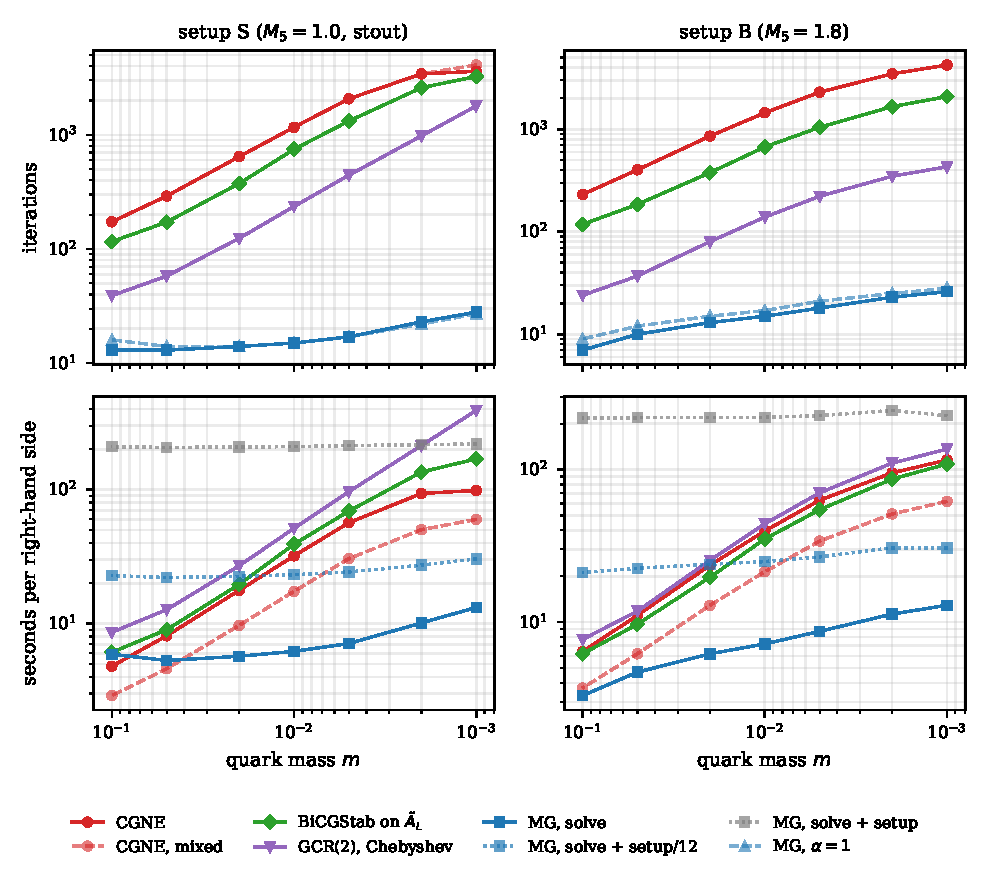
\includegraphics[width=\linewidth]{fig_massscan}
\caption{The mass scan of Table~\ref{tab:massscan}, the mixed-precision CGNE, and the Krylov
solvers on $\AL$ without the multigrid (Sec.~\ref{sec:nomg}): iterations (top) and seconds
per right-hand side (bottom) against the quark mass, $24^3\times48$. CGNE and multigrid: means over
the four configurations, bars from the smallest to the largest value; the solvers without the
multigrid: configuration~1. ``Solve + setup/12'': the setup spread over the 12 columns of one
point-source propagator.}
\label{fig:massscan}
\end{figure}

\paragraph{The reference solver.} It is CG on $\mathcal K\dg\mathcal K$, $\mathcal K=\Ce^{-1}S$,
the even-odd operator of Bridge++, with Neff's $\alpha$ as for the multigrid, in mixed precision.
Boyle and Yamaguchi~\cite{BY} used CG on $S\dg S$, which here needs more iterations
(Appendix~\ref{sec:cgform}).

\paragraph{Mass dependence.} The multigrid removes most of the critical slowing down of CGNE
(Fig.~\ref{fig:massscan}, Table~\ref{tab:massscan}). From $m=0.1$ to $m=0.001$ the iterations of
CGNE grow about twentyfold, those of the multigrid by $2.8$--$5.4$. Its setup is paid back after
$3.5$--$5.3$ right-hand sides at $m=0.001$. For $m\ge0.05$ in setup~S, CGNE is
faster or level. The multigrid needs three times the device memory of CGNE.

\paragraph{A point-source propagator.} At $m=0.001$ the multigrid takes $0.40$--$0.56$ of the wall
time of CGNE for a whole propagator, setup included (Table~\ref{tab:pointsource}). At $m=0.01$ the
setup is not quite paid back within the 12 columns. The pseudoscalar correlators of the two solvers
agree to $1\times10^{-6}$ or better.

\begin{table}[t]
\centering
\caption{Point-source propagators (12 columns) on $24^3\times48$: the multigrid
(setup seconds, iterations and seconds per column) against the mixed-precision CGNE
(iterations and seconds per column), the wall time of the whole propagator, and the
largest relative difference of the pseudoscalar correlator at $t=0\ldots3$. At $m=0.001$: ranges
over the four configurations and the 12 columns; at $m=0.01$: configuration~1.}
\label{tab:pointsource}
\renewcommand{\arraystretch}{1.12}
\setlength{\tabcolsep}{4pt}
\begin{tabular}{@{}lc ccc cc cc c@{}}
\toprule
 & & \multicolumn{3}{c}{MG} & \multicolumn{2}{c}{CGNE, mixed} & \multicolumn{2}{c}{wall (s)} & \\
\cmidrule(lr){3-5}\cmidrule(lr){6-7}\cmidrule(lr){8-9}
 & $m$ & setup & it & s & it & s & MG & CGNE & $|\Delta C|/C$\\
\midrule
S & $0.001$ & $203$--$222$ & $22$--$48$ & $11.1$--$26.4$ & $3634$--$6400$ & $52.1$--$91.6$ & $382$--$505$ & $678$--$1048$ & $\le1\times10^{-6}$\\
B & $0.001$ & $204$--$207$ & $22$--$30$ & $10.7$--$14.5$ & $4354$--$5574$ & $62.4$--$79.8$ & $363$--$398$ & $803$--$973$ & $\le7\times10^{-7}$\\
S & $0.01$ & $203$ & $16$--$17$ & $6.4$--$7.0$ & $1337$--$1388$ & $19.8$--$20.5$ & $305$ & $264$ & $2\times10^{-7}$\\
B & $0.01$ & $215$ & $17$ & $8.1$ & $1641$--$1745$ & $24.2$--$25.7$ & $331$ & $324$ & $4\times10^{-8}$\\
\bottomrule
\end{tabular}
\end{table}

\paragraph{Volume.} The advantage of the multigrid grows with the volume (Fig.~\ref{fig:volume},
Table~\ref{tab:volume}). It is slower than CGNE on $12^4$, about level on $16^4$, and clearly faster
from $24^4$ on: its iterations hardly grow with the volume, those of CGNE do. Its setup grows with
the volume.

\begin{figure}[t]
\centering
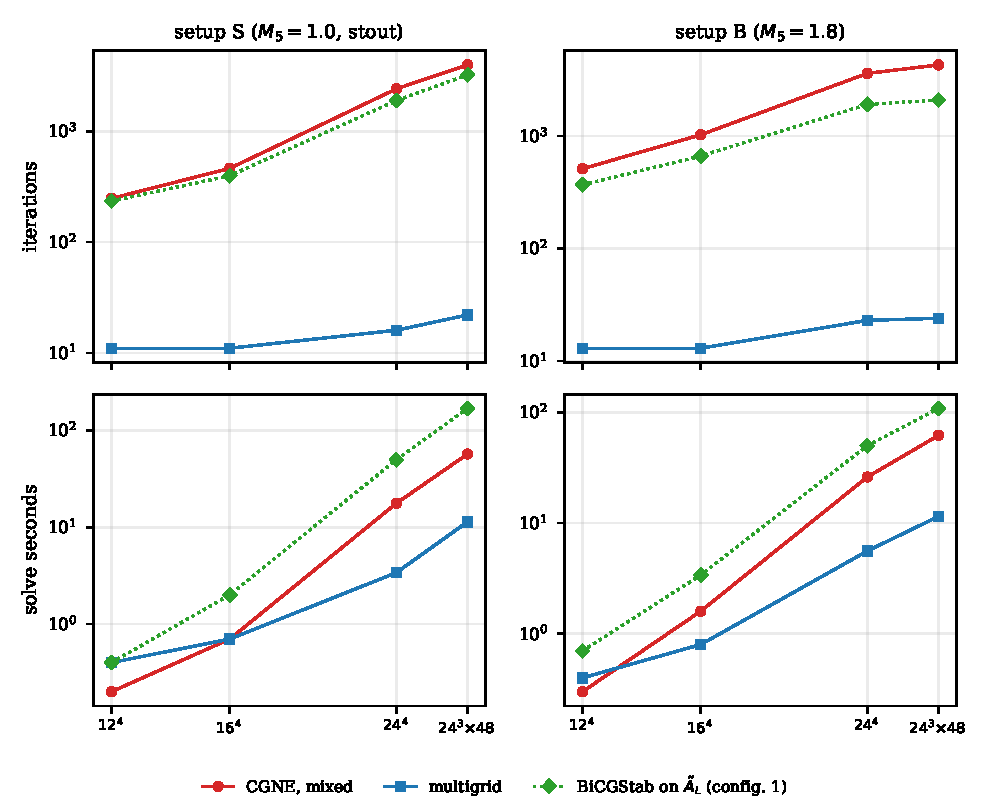
\includegraphics[width=\linewidth]{fig_volume}
\caption{Iterations (top) and solve seconds (bottom) at $m=0.001$ against the volume, one random
right-hand side. Mixed-precision CGNE and multigrid: median over the four configurations; BiCGStab
on $\AL$: configuration~1. The ranges are in Table~\ref{tab:volume}.}
\label{fig:volume}
\end{figure}



\paragraph{Neff's $\alpha$.} $\alpha=0.6$ saves CG far more iterations than the multigrid
(Table~\ref{tab:massscan}), as Sec.~\ref{sec:eo} expects.


\subsubsection{Solves with $D\dg$}
\label{sec:daggerresults}
\paragraph{Single solves.} Table~\ref{tab:c4} compares three ways to solve with $D\dg$ from one
setup of $D$. The right-hand sides are a random vector and the residual
$r=b-D\dg Dx_0$ after one sweep of the normal equations, solved to $10^{-10}$. The second kind
is the one that matters in HMC: its error lies mostly on the lowest modes.
\begin{itemize}
\item \emph{The cycle of $\AR\dg$ on the same $\Pro$} (the ``dual cycle''): the factorized
correction~\eqref{eq:corr} with $D$ and $\Dpv$ exchanged.
\item \emph{Flexible GCR on $D\dg$ with $\Gfive\mathcal M\Gfive$}, Eq.~\eqref{eq:c4}, one cycle a
step.
\end{itemize}

On $16^4$ the preconditioner $\Gfive\mathcal M\Gfive$ needs two to three iterations more than the solve
with $D$, in both setups and on both kinds of right-hand side, as the heuristic predicts. In
setup~S more inner cycles per step do not reduce the count, so the extra steps come from $N$ and
not from the inexact $\mathcal M$. The dual cycle stalls on the residual right-hand side in setup~S
on $12^4$ and on three of the four $16^4$ configurations.

On $12^4$ in setup~S, $m=0.001$, the residual right-hand side stalls GCR(2) on all four
configurations, and GCR(8) needs $13$--$222$ iterations. On $16^4$, where configurations 2--4 have
$Q=+1$, $+1$ and $+3$, GCR(2) needs $9$--$10$ on all four. The stall follows the small smeared
lattice of Sec.~\ref{sec:gcrk}, which we infer from the coincidence only: no $12^4$ run without smearing
was made for $D\dg$. The topological charge does not predict it. On the same right-hand side the
dual cycle does not converge on $12^4$ in setup~S.

\paragraph{What did not work.} None of the other ways we tried to solve with $D\dg$ from one setup
is as good as $\Gfive\mathcal M\Gfive$. The exact map of Eq.~\eqref{eq:g5exact} needs $D_-^{-1}$,
which does not converge (Sec.~\ref{sec:g5fail}). For the dual cycle, $\Pro$ from $y\cup\Gfive y$
converges but quadruples the coarse operators, other prolongations need up to $300$ iterations, and
GCR(4) in place of BiCGStab for its Pauli--Villars factor converges at three times the cost per
cycle.

\paragraph{What these solves are for.} In HMC each force evaluation needs one solve with $D$ and one
with $D\dg$, and with $\Gfive\mathcal M\Gfive$ one setup serves both. The cost in HMC is left to
future work (Sec.~\ref{sec:open}).


\subsection{What each part contributes}
\label{sec:parts}

The speed-up of Sec.~\ref{sec:massscan} rests on four choices beyond the operator $A'$: the coarse
correction, the lift $\hat t$ in the basis, the regularized Pauli--Villars solve,
and the setup parameters. Each part below isolates one of them.

\subsubsection{Krylov on $\AL$ without the multigrid}
\label{sec:nomg}

The speed-up comes from the coarse correction: without it a Krylov method on $\AL$ does not beat
CGNE (Fig.~\ref{fig:massscan}). BiCGStab on $\AL$ alone needs about as many iterations as
double-precision CGNE, but each of its iterations applies $\AL$ twice, so it takes longer. The
Chebyshev smoother as a preconditioner cuts its iterations but raises the time.


\subsubsection{Choice of the prolongation basis}
\label{sec:basischoice}
The exactness~\eqref{eq:exact} needs both lifts $s$ and $\hat t$ of each $y$ in
$\operatorname{range}\Pro$, but the left form used in practice is not exact
(Sec.~\ref{sec:basis}). To see what $\hat t$ does there, we replace it by $Ds$, which
vanishes on the odd sites, or drop it (Table~\ref{tab:basischoice}). With $\{s\}$ alone $\Pro$
has half the columns; to compare at the same size we also take $32$ vectors $y$, which doubles
the vectors of the filter and of the bootstrap.


With the same vectors $y$, the two lifts give the fewest iterations on every volume. In setup~S,
replacing $\hat t$ by $Ds$ or dropping it stagnates on three of the four $12^4$ and $16^4$
configurations and costs five times the iterations on $24^3\times48$; in setup~B it costs more
iterations. Twice as many vectors $y$ with $\{s\}$ alone take the place of $\hat t$ on
$24^3\times48$ but not on $12^4$, at a longer setup and twice the host memory; a point-source
propagator is still faster with the two lifts.

\subsubsection{The regularized Pauli--Villars solve}
\label{sec:pvcoarse}

With the regularized solve no slow setups remain on $12^4$: all $40$ setups of setup~S need
$10$--$17$ iterations, against $70$ to more than $2000$ for the slow ones without it
(Table~\ref{tab:tikhonov}). The cause is the Galerkin factor. With stout smearing its smallest
singular value is $1/79$ to $1/15$ of that of the fine $\Dpv$ on the four configurations; without
smearing the two agree to within $4\%$ (Table~\ref{tab:pvsv}).

\subsubsection{Sensitivity to the parameters}
\label{sec:sensitivity}


The method is robust within a window of each parameter and fails outside it
(Fig.~\ref{fig:sensitivity}). The smoother interval must suit the
setup, the bootstrap is necessary, and more accurate coarse solves do not help.

\begin{figure}[t]
\centering
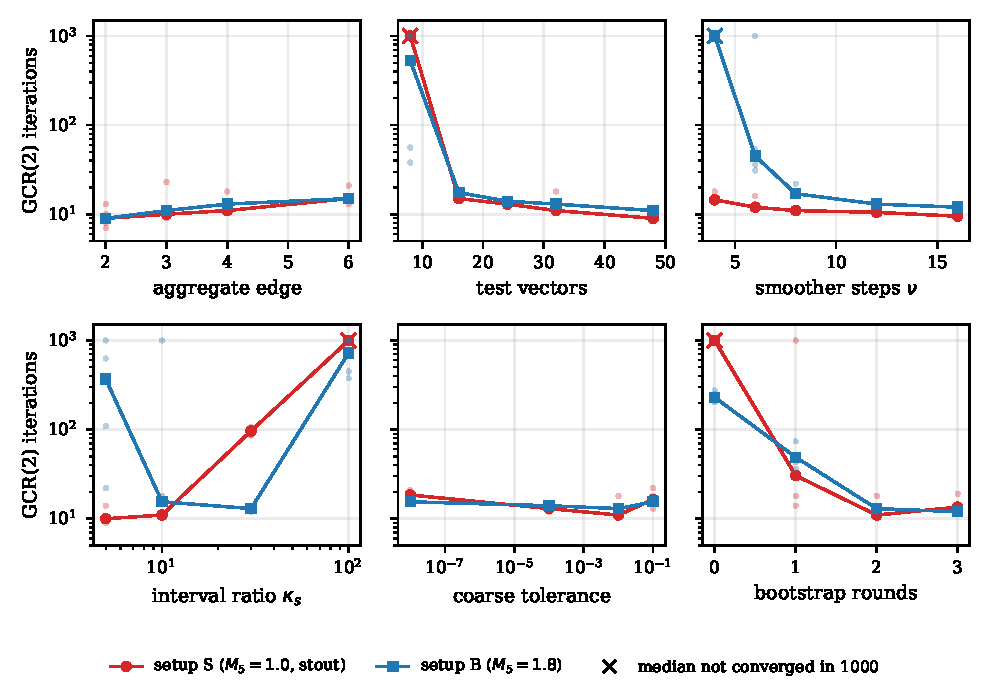
\includegraphics[width=\linewidth]{fig_sensitivity}
\caption{GCR(2) iterations on $\AL$ when one parameter of Table~\ref{tab:setups} is changed,
$12^4$, $m=0.001$, one random right-hand side. Lines: median over the four configurations; dots: the
four configurations; a cross marks a median that does not converge in $1000$ iterations. The default
is the point where the lines of the two setups pass through $14$ iterations. Values and setup and solve
times in Table~\ref{tab:costs}.}
\label{fig:sensitivity}
\end{figure}



Fewer iterations are not always less time (Table~\ref{tab:costs}). Smaller aggregates and more test
vectors save iterations, but the larger coarse space makes the setup and each iteration longer.
On $24^3\times48$, $16$ test vectors do not suffice: the solve needs hundreds of iterations or does
not converge in $2000$. Outside the window the failures can come from the outer solver alone. With
$\kappa_s=10$ in setup~B, one of the four $12^4$ configurations brings GCR(2) to a plateau; with the
same cycle GCR(16) converges, and other setup seeds converge with GCR(2).

Whyte, Stathopoulos and Romero~\cite{WhyteSVD} obtain, for Wilson fermions, the effect of more test
vectors at the coarse size of fewer by truncating them with a singular value decomposition on each
aggregate. Here the truncated basis would no longer contain $s$ and $\hat t$ exactly; whether the
gain outweighs that loss is open.

\subsection{Why the method converges}
\label{sec:why}

The convergence is set by the spectrum and the pseudospectra of the preconditioned operator, not
by its field of values. On the smeared lattices the field of values of $\AR\mathcal M$ reaches into
the left half-plane, so the bound of Eisenstat, Elman and Schultz~\cite{ESS} for GCR does not apply.
Its eigenvalues lie at $\Re\lambda\ge0.70$ with moderate condition numbers, and its pseudospectra
bound full GMRES. As usual for multigrid preconditioners of lattice Dirac operators, the
convergence of the truncated flexible outer method is established numerically.

Two notions from non-Hermitian linear algebra are used. The \emph{field of values}
$W(X)=\{z\dg Xz/z\dg z\}$ contains the spectrum, and its leftmost point is the smallest eigenvalue
of the Hermitian part $(X+X\dg)/2$; GCR converges at every restart length when $W$ lies in the
right half-plane~\cite{ESS}. The \emph{$\varepsilon$-pseudospectrum} is the set of $z$ where
$\sigma_{\min}(z-X)<\varepsilon$; for a normal $X$ it is the $\varepsilon$-neighborhood of the
spectrum, for a non-normal one it can be much larger, and it bounds full
GMRES~\cite{TrefethenEmbree}. The condition number of an eigenvalue, $\kappa=1/|y\dg x|$ for its
normalized right and left eigenvectors, is $1$ for a normal matrix and widens the pseudospectrum
around the eigenvalue.

The quantities of this subsection take $\mathcal M$ as a fixed linear map: both coarse factors solved
to $|r|^2/|b|^2<10^{-20}$ in double precision, the Pauli--Villars factor regularized as in
Eq.~\eqref{eq:tikhonov}, and $\mathcal M\dg$ built as its adjoint, so that
$\langle z|\AR\mathcal M w\rangle$ and $\langle\mathcal M\dg\AR\dg z|w\rangle$ agree to $10^{-10}$.

\subsubsection{Field of values: the coarse correction amplifies}
\label{sec:fov}

The coarse correction pushes the field of values into the left half-plane (Table~\ref{tab:fov}).
The field of values of $\AR$ itself reaches only just below zero and hardly depends on the volume,
and the smoother is harmless, $\|I-\AR\mathcal S\|\approx1$. The coarse correction $E$ is the identity
on the vectors it is built from (Eq.~\eqref{eq:exact}) but amplifies other directions, like a
strongly oblique projection, by three orders of magnitude. The post-smoothing acts as a filter
and brings the whole cycle back close to the identity. Eick and Mawhinney~\cite{EickMawhinney}
describe the same mechanism for a renormalization-group coarse lattice and need a Chebyshev filter
of high degree; here $\AR$ is close to the identity on the high modes, and the smoother suffices.

With stout smearing $W(\AR\mathcal M)$ crosses the origin on every configuration. Without smearing
the amplification is far smaller and $W(\AR\mathcal M)$ lies in the right half-plane, where
truncated GCR($k$) is guaranteed to converge for every $k$~\cite{ESS}.

\subsubsection{Spectrum: far from the origin}
\label{sec:spectrum}

The spectrum, unlike the field of values, stays far from the origin (Table~\ref{tab:spectrum},
Fig.~\ref{fig:spectrum}). Every eigenvalue lies at $\Re\lambda\ge0.70$, with moderate condition
numbers. Setup~S has one or two isolated outliers of larger modulus, and all other eigenvalues lie in
a disc about $1$ that excludes the origin. The left and right forms have nearly the same spectrum.

\subsubsection{Pseudospectra and a bound for GMRES}
\label{sec:pseudo}

For a non-normal operator the eigenvalues alone do not bound the convergence of
GMRES; the $\varepsilon$-pseudospectrum, the set where $\sigma_{\min}(z-X)<\varepsilon$,
does~\cite{NRT,TrefethenEmbree}. If a contour $\Gamma$ of length $L$ encloses the
spectrum of $X$ but not the origin and $\sigma_{\min}(z-X)\ge\varepsilon$ on it, then
for any polynomial $p_k$ with $p_k(0)=1$,
\begin{equation}
\frac{\|r_k\|}{\|r_0\|}\le\|p_k(X)\|\le\frac{L}{2\pi\varepsilon}\max_{z\in\Gamma}|p_k(z)| .
\label{eq:pseudobound}
\end{equation}
An isolated outlier $\lambda_o$ outside $\Gamma$ is removed by the factor
$(1-z/\lambda_o)$ of $p_k$: then $p_k(X)=p_k(X)(I-P_o)$ with $P_o$ the spectral
projector, $\|(z-X)^{-1}(I-P_o)\|\le\kappa_o/\varepsilon$, and with a circle
$|z-c|=r$ and $p_k(z)=(1-z/\lambda_o)(1-z/c)^{k-1}$,
\begin{equation}
\frac{\|r_k\|}{\|r_0\|}\le\kappa_o\,\frac{r}{\varepsilon}\,
\frac{|\lambda_o-c|+r}{|\lambda_o|}\Big(\frac rc\Big)^{k-1}.
\label{eq:outlierbound}
\end{equation}

\begin{figure}[t]
\centering
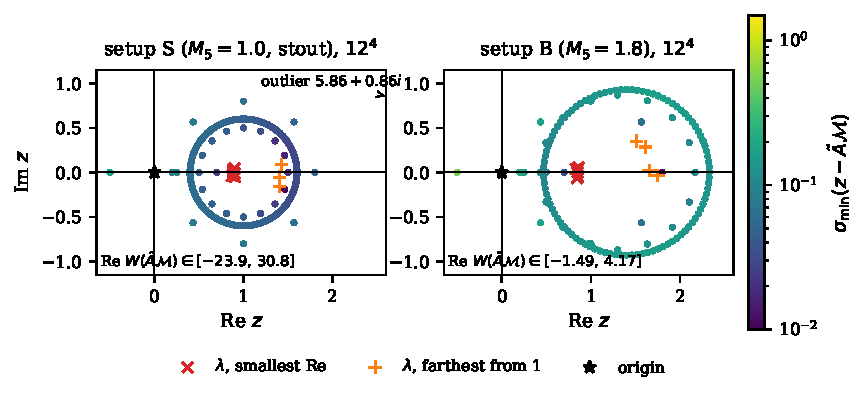
\includegraphics[width=\linewidth]{fig_spectrum}
\caption{$12^4$, $m=0.001$, exact coarse solves (the Pauli--Villars factor regularized): the six eigenvalues of
$\AR\mathcal M$ of smallest real part, the four farthest from $1$, and
$\sigma_{\min}(z-\AR\mathcal M)$ (color) at the points where it was computed: the contours of
Table~\ref{tab:pseudo}, among them the dense circles $|z-1|=0.6$ (S) and
$|z-1.4|=0.93$ (B). The field of values reaches far into the left half-plane (its real
range in the corner), the spectrum does not.}
\label{fig:spectrum}
\end{figure}

On $16^4$ setup~S has two outliers; the factor $\kappa_o$ is then replaced by
$\|I-P_1-P_2\|\le1+\kappa_1+\kappa_2$ and there are two factors of the form
$(|\lambda_o-c|+r)/|\lambda_o|$. On the dense circles of $12^4$ the spacing of the points is small
enough that, $\sigma_{\min}(z-X)$ being $1$-Lipschitz in $z$, the bound holds on the whole circle; it
guarantees $\|r_k\|/\|r_0\|<10^{-9}$ within $55$ (S) and $57$ (B) iterations (Table~\ref{tab:pseudo}).

The bound guarantees convergence at a fixed rate, $r/c$ per iteration, with no stagnation. Its rate,
$r/c=0.5$--$0.6$ in setup~S, is close to the one we measure on $24^3\times48$ on configurations 1 and
3, where the median factor per GCR step of $|r|^2$ is $0.23$--$0.41$ (Fig.~\ref{fig:history}), that
is $0.48$--$0.64$ in $|r|$; configuration~2 in setup~S converges more slowly. The Lanczos estimates approach $\sigma_{\min}^2$ from above, the disc rests on the
eigenvalues farthest from $c$ found by Arnoldi, and the bound is for full GMRES with a fixed
$\mathcal M$.

\subsubsection{Truncated GCR and inexact coarse solves}
\label{sec:gcrk}

Truncated GCR does not need accurate coarse solves. With the usual coarse solves to $10^{-2}$,
GCR(2) needs at most one iteration more than GCR(32) on $12^4$ (Table~\ref{tab:gcrk}). Coarse solves
to $10^{-8}$, where $\mathcal M$ is close to the fixed map, do not help: GCR(2) then needs $19$
iterations and GCR($\ge16$) $15$.

Where $E$ amplifies, the solver's cycle is better than the fixed map. At the vector $x$ at the left
end of $W(\AR\mathcal M)$, coarse solves to $10^{-2}$ reduce $\|(I-\AR E)x\|$ by large factors against
exact ones and in most cases make $\Re\,x\dg\AR\mathcal Mx$ positive. With Krylov coarse solves stopped
early the cycle is not a fixed linear map, so this holds for these vectors only.

A truncated method has no guarantee when the field of values contains the origin~\cite{ESS,Embree}.
With a fixed cycle GCR(2) can reach a fixed point, where the new direction is orthogonal to the
residual and the next step repeats it. With the parameters of Table~\ref{tab:setups} no run reached
a plateau. The one plateau we checked, at $\kappa_s=10$ in setup~B (Sec.~\ref{sec:sensitivity}), is
of this kind: the same cycle converges with GCR(16).

\paragraph{Setup seeds.} With the regularized Pauli--Villars solve no setup is slow on $12^4$
(Sec.~\ref{sec:pvcoarse}). Configuration~2 of $24^3\times48$ needs more iterations than the other
three (Table~\ref{tab:volume}); which property of that configuration causes this is open.

\begin{figure}[t]
\centering
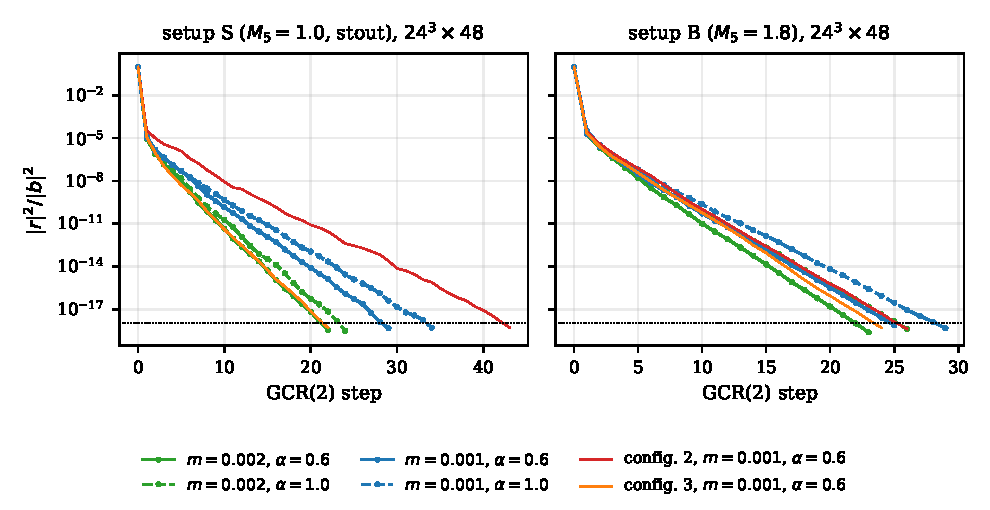
\includegraphics[width=\linewidth]{fig_history}
\caption{GCR(2) residual histories on $24^3\times48$, $\AL$, the multigrid of Table~\ref{tab:setups}: configuration~1 (blue, green) and configurations 2 and 3 at $m=0.001$, $\alpha=0.6$ (red, orange).}
\label{fig:history}
\end{figure}

On $24^3\times48$ no run shows a plateau (Fig.~\ref{fig:history}).


% ============================================================
\section{Summary}
\label{sec:summary}

Boyle and Yamaguchi named three reasons why the Pauli--Villars multigrid did not beat red-black
CG in four-dimensional QCD: it worked on the whole lattice, its coarse space kept the fifth
dimension, and its non-normal coarse solves were not deflated. The present method addresses them
in turn. It solves the even-odd system. Its aggregates contain the whole fifth dimension, so the
correction solves two nearest-neighbor systems on a four-dimensional coarse lattice. Its
Pauli--Villars coarse system is solved in a $\Sigma$-Hermitian form, and levels below the coarse
lattice take the place of deflation. With the same test vectors, the lift $\hat t$ that makes the
correction exact for the right form cuts the iterations by up to a factor of $22$ also in the
left form, which is not exact; one lift of twice as many vectors matches it on $24^3\times48$ at
$1.6$--$1.8$ times the setup time.

On quenched configurations on one GPU the multigrid iterations on $24^3\times48$ grow by a factor
of $2$--$4$ from $m=0.1$ to $m=0.001$, against $20$ for even-odd CGNE. At $m=0.001$ a solve is
faster than with mixed-precision CGNE from $24^4$ on, by $4.5$--$4.8$ on $24^3\times48$, and a
point-source propagator takes half the time, setup included. One setup serves Neff's $\alpha$ and
the solves with $D\dg$, and the multigrid runs in HMC. The field of values of the preconditioned
operator reaches into the left half-plane; its spectrum and pseudospectra account for the
convergence.

The evidence is limited to one configuration per volume, volumes up to $24^3\times48$, and CGNE as
the only reference solver. A comparison with HDCG and with the coarsening of $\Dpv\dg D$ in one
implementation, and larger volumes, are the next steps (Sec.~\ref{sec:open}). For propagators,
applying the coarse operators and the transfer to the 12 columns of a point source together would
raise their intensity from about one flop per byte to about ten, as for Wilson-clover
multigrid~\cite{Grebe}; a solve in HMC, with one right-hand side, would not gain from it.

\paragraph{Code and data.} All results were obtained with RutticeQCD,
\url{https://github.com/atsanroger/RutticeQCD}, whose GPU backend takes the CUDA kernels of the
Wilson and M\"obius operators from Bridge++. The parameter files, the data of the tables and
figures and the scripts that make them are in \texttt{docs/mg\_background} of the repository,
with a guide to reproducing the results (\texttt{REPRODUCE.pdf}) and a line-by-line derivation of
the formulas (\texttt{MG\_WALKTHROUGH.pdf}).
\fi
% ============================================================
\section{Open problems}
\label{sec:open}

\ifresults
The following questions remain open. Those the measurements answer are discussed where
they arise: the left form in Sec.~\ref{sec:basis}, $c\neq0$ in Secs.~\ref{sec:coarse}
and \ref{sec:herm}, the field of values in Secs.~\ref{sec:spectra} and
\ref{sec:fov}--\ref{sec:pseudo}.

\begin{enumerate}
\item \textbf{Parameters from the operator.} The smoother interval
$[\lambda_{\rm hi}/\kappa_s,\lambda_{\rm hi}]$ uses a ratio chosen per setup, and a wrong one makes
the solve stagnate (Sec.~\ref{sec:sensitivity}); the setup works with singular values of $\AR$,
which for a non-normal operator need not match its eigenvalues. How to set the interval from the
operator, and whether an ellipse with complex foci should replace the real interval, is open. So
is the number of test vectors. Local coherence suggests that it does not grow with the volume,
yet $16$ suffice on $12^4$ and $24$ do not on $24^3\times48$ (Sec.~\ref{sec:sensitivity}). The
low modes may vary in the fifth dimension more than one vector per aggregate can follow (Eick and
Mawhinney~\cite{EickMawhinney} find their fifth-dimensional profiles to differ between
lattices); a test vector split in $s$, as it is now split in chirality, would keep $s$ and
$\hat t$ in the range of $\Pro$, and Lüscher's coherence test would measure what the coarse space
captures.

\item \textbf{Convergence theory.} The pseudospectral bound rests on Lanczos estimates of
$\sigma_{\min}$, which approach it from above, and on the eigenvalues farthest from the center
found by Arnoldi (Sec.~\ref{sec:pseudo}). A bound from an inclusion theorem, and how the outliers
of setup~S and the pseudospectra develop beyond $16^4$, are open; on $24^4$ the Arnoldi iteration
does not fit in $24$\,GB of device memory. No theory covers truncated GCR with a preconditioner that
varies from step to step. On the $12^4$ configuration GCR(2) with accurate coarse solves reaches a
residual orthogonal to its new direction and stays there (Sec.~\ref{sec:gcrk}), and the residual
right-hand side of HMC needs GCR(8) for $D\dg$ (Sec.~\ref{sec:daggerresults}). GCR(2) does not
reach such a fixed point on $16^4$ and $24^4$, although $24^4$ has $Q=+4$; the solves with $D\dg$
were tested on $16^4$ but not on $24^4$. What singles out this configuration is open. A safeguard that changes the
direction when $|\langle r,\tilde A\mathcal Mr\rangle|/(\|r\|\,\|\tilde A\mathcal Mr\|)$ falls
below a threshold would remove such fixed points for one inner product per step; it has not been
implemented. Why $N=c[Y,W]D^{-1}$ has a small square, beyond the heuristic of
Sec.~\ref{sec:dagger}, is open as well.

\item \textbf{Formulations and coarse spaces.} The comparison here is with CGNE. How the two
nine-point factors compare with the $81$-point HDCG operator and with the $33$-point coarsening of
$\Dpv\dg D$~\cite{BoyleOare}, in cost per iteration and in iterations, needs all of them in one
code on the same lattices. The same holds for the full-lattice $A'$ against the even-odd system.
Boyle and Yamaguchi~\cite{BY} found a red-black smoother ineffective with the HDCR correction,
because the eigenvectors of the red-black operator and of $\gamma_5RD$ are not aligned; here the
smoother and the correction both approximate $\tilde A^{-1}$, so that mismatch is absent by
construction, but whether the even-odd system is preferable for this method has not been
established. Finally, $\Pro$ and the coarse operators are those of the plain $D$ and $\Dpv$;
whether a $\Pro$ built from the near-null vectors of $D^{(\alpha)}$, $Q^{-1}$ times those of $D$,
helps the left form with $\alpha$ has not been tried.
\end{enumerate}
\else
The following questions of theory and algorithm remain open.

\begin{enumerate}
\item \textbf{Exactness for the left form.} Proposition~\ref{prop:exact} holds
for the right form. For $\AL$ (with or without $\alpha$) the Pauli--Villars lift
that would be needed differs from $\hat t$ by site-local factors (second remark
of Sec.~\ref{sec:basis}). Whether a basis can be made exact for both forms at
once, and what is lost by using the right-form basis for the left form, is open.

\item \textbf{Loss of $\Gfive$-Hermiticity for $c\neq0$.} By
Eq.~\eqref{eq:g5herm}, $\Gfive D\Gfive\neq D\dg$ at $O(c)$. MINRES on
$\Hc=\Dcpv\Sigma$, the absolute-value block preconditioner (built from the
Hermitian part only), the additive level preconditioner, and the $\Sigma$-adjoint
in place of the exact adjoint are all exact only for $c=0$. The exactly Hermitian
operator $\Gfive D_-^{-1}D$~\cite{BNO} involves a non-local inverse. How large
the non-Hermitian part is on the coarse space, and how to treat it, is open.

\item \textbf{Smoother interval for a non-normal operator.} The interval
$[\lambda_{\rm hi}/\kappa_s,\lambda_{\rm hi}]$ is set from an estimate of the
spectral radius, whereas the setup works with singular values (eigenvalues of
$\AR\dg\AR$). For a non-normal $\tilde A$ these need not agree. Which part of
the low end is left to the smoother after the coarse correction, and whether an
ellipse with complex foci should replace the real interval, are open.

\item \textbf{Even-odd smoother and coarse space.} Boyle and
Yamaguchi~\cite{BY} found that a red-black smoother combined with the HDCR
coarse correction was not effective, and attributed it to the eigenvectors of
the red-black operator and of $\gamma_5RD$ not being aligned. In the present
method the smoother and the correction both approximate $\tilde A^{-1}$ and the
coarse space is built from low modes of $\AR$, so that particular mismatch is
absent by construction; but the coarse operators are Galerkin projections of
$D$ and $\Dpv$, not of $\tilde A$. Whether the even-odd outer system is
preferable to the full-lattice $A'$ for this method has not been established.

\item \textbf{Field of values versus real parts of eigenvalues.}
Section~\ref{sec:spectra} shows $\Re\lambda>0$ for $A'$. The GCR bound~\cite{ESS}
needs a positive definite Hermitian part, i.e.\ a field of values in the right
half-plane, which is a stronger condition. Whether it holds for $A'$, $\AR$ and
$\AL$, and whether a shift of the kind used in Ref.~\cite{BoyleOare} is needed,
is not known.

\item \textbf{Outer solver with a varying preconditioner.} Because the coarse
solves are truncated, $\mathcal M$ is nonlinear and depends on the right-hand
side. FGMRES and flexible GCR allow this; BiCGStab does not, and its behavior
with $\mathcal M$ as preconditioner has no theoretical justification.

\item \textbf{Solving with $D\dg$.} Sec.~\ref{sec:dagger} uses $\Gfive D^{-1}\Gfive$ as a
preconditioner of $D\dg$; its error $N=c[Y,W]D^{-1}$ is argued to have a small square. A
bound on $\|N^2\|$ on the low modes has not been derived.
\end{enumerate}

\fi
% ============================================================
\clearpage
\appendix
\begin{center}\Large\bfseries Appendices\end{center}
\addcontentsline{toc}{section}{Appendices}
\renewcommand{\theequation}{\thesection.\arabic{equation}}

\section{The notation of other references}
\label{sec:notation}
Table~\ref{tab:notation} relates Eqs.~\eqref{eq:Y}--\eqref{eq:Q} to Brower, Neff
and Orginos~\cite{BNO}, to Kanamori, Chen and Matsufuru~\cite{KCM2024} and to the
code of Bridge++~\cite{Bridge} (\texttt{Fopr\_Domainwall}, \texttt{Fopr\_Domainwall\_eo},
with Neff's $\alpha$ as \texttt{parameter\_alpha}). Eq.~\eqref{eq:Dslice} is the
tridiagonal matrix of Ref.~\cite{BNO}, Eq.~(2.20), and of Ref.~\cite{KCM2024}, Eq.~(1), with
$D_+=1+bW$ on the diagonal, $D_-\Pp$ below and $D_-\Pm$ above it, $-mD_-P_\pm$ in the corners,
and $s$ shifted by one. The operators $D$, $C$ and $D^{(\alpha)}$ are thus the same in all four;
the differences are names and signs:
\begin{itemize}
\item $D_\pm$ are those of Refs.~\cite{BNO,KCM2024}, $D_-=cW-1$. The hop $Y$ of
Eq.~\eqref{eq:Y} carries a minus sign, so $D=D_+-D_-Y$ and $d_-=1-c(4-M_5)$ is minus the
site part of $D_-$. The comments of RutticeQCD on the five-dimensional source call $1-cW$
``$D_-$'', which is $-D_-$ (the source is that of the Bridge++ domain-wall test, sign
included).
\item The height $M_5>0$ here is $M_0$ in Ref.~\cite{KCM2024} and in Bridge++
(\texttt{domain\_wall\_height}); Ref.~\cite{BNO} writes $M_5$ for the Wilson mass,
$M_5^{\mathrm{BNO}}=-M_5$, Eq.~(2.13). The caption of Fig.~1 of Ref.~\cite{KCM2024}
gives $M_0=-1$ for the height $1$ of its text.
\item The $\alpha$ of Ref.~\cite{BNO}, $(b+c)/(b-c)$, is the scale factor of the
M\"obius kernel ($2$ at $b=1.5$, $c=0.5$), not Neff's $\alpha$ of Eq.~\eqref{eq:Q}.
\item $\Gamma_5=\gamma_5RD_-^{-1}$ in Ref.~\cite{BNO}, Eq.~(2.22); here $\Gfive=\gamma_5R$.
\end{itemize}
$D^{(\alpha)}$ here and the operator of Bridge++ with \texttt{parameter\_alpha} were
compared on a $12^4$ configuration with stout links, $L_s=8$, $m=0.01$: at $\alpha=0.6$
and $\alpha=1$ CG on the even-odd normal equation took the same number of iterations
for every column of a point source, and the pseudoscalar correlators agree to
$10^{-11}$. Bridge++ returns $\psi^{(\alpha)}$; $\psi=Q\psi^{(\alpha)}$.

\begin{table}[t]
\centering
\caption{The notation of this paper (and of RutticeQCD) and that of other references.
Equation numbers are those of the references; ``the same'' means the same operator.}
\label{tab:notation}
\footnotesize
\setlength{\tabcolsep}{3pt}
\renewcommand{\arraystretch}{1.15}
\begin{tabular}{@{}>{\raggedright}p{1.7cm}>{\raggedright}p{3.0cm}>{\raggedright}p{3.1cm}>{\raggedright}p{2.9cm}>{\raggedright\arraybackslash}p{3.6cm}@{}}
\toprule
 & This paper & Ref.~\cite{BNO} & Ref.~\cite{KCM2024} & Bridge++ code\\
\midrule
Height & $M_5>0$ & $-M_5$, $M_5=O(-1)$ (2.13) & $M_0$ & $M_0$, \texttt{domain\_wall\_height}\\
Fifth dim. & $s=0,\dots,L_s-1$ & $s=1,\dots,L_s$ & $s=1,\dots,N_s$ & $0,\dots,N_s-1$, \texttt{extent\_of\_5th\_\allowbreak dimension}\\
Wilson part & $W=(4-M_5)-\tfrac12K$ & $D^{\mathrm{Wilson}}(M_5)$ (2.13) & $D_{\mathrm W}(-M_0)$ & $\frac1{2\kappa}D_{\mathrm W}$, $\kappa=1/(8-2M_0)$\\
$D_\pm$ & $D_+=1+bW$, $D_-=cW-1$ (Eq.~\eqref{eq:Dpm}) & $D_+=bD^{\mathrm{W}}+1$, $D_-=cD^{\mathrm{W}}-1$ (2.18) & the same (2) & ---\\
$D$ & Eq.~\eqref{eq:D} & $D_{\mathrm{DW}}(m)$ (2.20) & $D(m)$ (1) & \texttt{Fopr\_Domainwall}, mode \texttt{D}\\
$C$ & $d_++d_-Y$, Eq.~\eqref{eq:Cblocks} & --- & $\mathrm{diag}(D_{ee},D_{oo})$ (4) & $D_{ee}$, $D_{oo}$ of \texttt{\_eo}; \texttt{m\_dp}${}=\alpha d_+$, \texttt{m\_dm}${}=\alpha d_-$\\
Neff's $\alpha$ & $DQ$, Eq.~\eqref{eq:Q} & --- (its $\alpha=\frac{b+c}{b-c}$) & --- & \texttt{parameter\_alpha}: $DQ$, site part $CQ$\\
$\Gamma_5$ & $\gamma_5R$ & $\gamma_5RD_-^{-1}$ (2.22) & --- & ---\\
4d quark & $\Pm\psi_0+\Pp\psi_{L_s-1}$ & $P_-\Psi_1$, $P_+\Psi_{L_s}$ & --- & the same\\
\bottomrule
\end{tabular}
\end{table}

\ifresults
\ifresults
% ============================================================
\section{Gauge configurations}
\label{sec:configs}

All quenched configurations use the plaquette gauge action at $\beta=6.0$ and were generated by
the HMC of RutticeQCD from a cold start, 400 trajectories of length $0.5$ (on $24^3\times48$, 400
from a cold start and then 200). The dynamical $16^4$ configuration was thermalized from the
quenched one by the HMC of setup~S (Sec.~\ref{sec:hmcresults}). Table~\ref{tab:configs}
gives the plaquette, the scale $t_0$ ($t^2E=0.3$, $E$ of the clover field strength) and the
topological charge at $t_0$ after the Wilson flow (step $0.01$), of the clover field strength and
improved with rectangles ($c_{\rm plaq}=5/3$, $c_{\rm rect}=-1/12$). On the larger lattices the
two definitions differ by up to $1$ at $t_0$.

\begin{table}[h]
\centering
\caption{The gauge configurations: plaquette, $t_0/a^2$, and the topological charge at $t_0$.
\texttt{ruttice-flow}; the logs and the generation histories are listed with the data.}
\label{tab:configs}
\renewcommand{\arraystretch}{1.12}
\begin{tabular}{@{}lccccc@{}}
\toprule
lattice & plaquette & $t_0/a^2$ & $Q_{\rm clover}$ & $Q_{\rm imp}$ & $Q$\\
\midrule
$12^4$ & $0.594250$ & $3.19$ & $+0.94$ & $+1.00$ & $+1$\\
$16^4$ & $0.593509$ & $3.54$ & $+0.05$ & $+0.01$ & $0$\\
$16^4$ dynamical & $0.593809$ & $6.90$ & $-0.003$ & $-0.0002$ & $0$\\
$24^4$ & $0.593524$ & $3.65$ & $+3.63$ & $+3.92$ & $+4$\\
$24^3\times48$ & $0.593548$ & $3.20$ & $+4.47$ & $+4.78$ & $+5$\\
$32^4$ & $0.593606$ & $3.59$ & $+13.0$ & $+14.1$ & $\approx+14$\\
\bottomrule
\end{tabular}
\end{table}

\fi
\fi

% ============================================================
\begin{thebibliography}{99}
\bibitem{RBCKpipi} R.~Abbott \emph{et al.} (RBC and UKQCD), \emph{Direct CP violation and the $\Delta I=1/2$ rule in $K\to\pi\pi$ decay from the Standard Model}, Phys.\ Rev.\ D \textbf{102} (2020) 054509 [arXiv:2004.09440].
\bibitem{RBCHVP} T.~Blum \emph{et al.} (RBC and UKQCD), \emph{Calculation of the hadronic vacuum polarization contribution to the muon anomalous magnetic moment}, Phys.\ Rev.\ Lett.\ \textbf{121} (2018) 022003 [arXiv:1801.07224].
\bibitem{RBCWindow} T.~Blum \emph{et al.} (RBC and UKQCD), \emph{An update of Euclidean windows of the hadronic vacuum polarization}, Phys.\ Rev.\ D \textbf{108} (2023) 054507 [arXiv:2301.08696].
\bibitem{RBCHLbL} T.~Blum, N.~Christ, M.~Hayakawa, T.~Izubuchi, L.~Jin, C.~Jung and C.~Lehner, \emph{The hadronic light-by-light scattering contribution to the muon anomalous magnetic moment from lattice QCD}, Phys.\ Rev.\ Lett.\ \textbf{124} (2020) 132002 [arXiv:1911.08123].
\bibitem{JLQCDBpi} B.~Colquhoun, S.~Hashimoto, T.~Kaneko and J.~Koponen, \emph{Form factors of $B\to\pi\ell\nu$ and a determination of $|V_{ub}|$ with M\"obius domain-wall fermions}, Phys.\ Rev.\ D \textbf{106} (2022) 054502 [arXiv:2203.04938].
\bibitem{HashimotoInclusive} S.~Hashimoto, \emph{Inclusive semi-leptonic $B$ meson decay structure functions from lattice QCD}, PTEP \textbf{2017} (2017) 053B03 [arXiv:1703.01881].
\bibitem{GambinoInclusive} P.~Gambino, S.~Hashimoto, S.~M\"achler, M.~Panero, F.~Sanfilippo, S.~Simula, A.~Smecca and N.~Tantalo, \emph{Lattice QCD study of inclusive semileptonic decays of heavy mesons}, JHEP \textbf{07} (2022) 083 [arXiv:2203.11762].
\bibitem{BaroneInclusive} A.~Barone, S.~Hashimoto, A.~J\"uttner, T.~Kaneko and R.~Kellermann, \emph{Approaches to inclusive semileptonic $B_{(s)}$-meson decays from lattice QCD}, JHEP \textbf{07} (2023) 145 [arXiv:2305.14092].
\bibitem{NarayananNeuberger} R.~Narayanan and H.~Neuberger, \emph{Infinitely many regulator fields for chiral fermions},
Phys.\ Lett.\ B \textbf{302} (1993) 62 [hep-lat/9212019].
\bibitem{Neuberger} H.~Neuberger, \emph{Exactly massless quarks on the lattice},
Phys.\ Lett.\ B \textbf{417} (1998) 141 [hep-lat/9707022].
\bibitem{Kaplan} D.~B.~Kaplan, \emph{A method for simulating chiral fermions on the lattice},
Phys.\ Lett.\ B \textbf{288} (1992) 342 [hep-lat/9206013].
\bibitem{Shamir} Y.~Shamir, \emph{Chiral fermions from lattice boundaries},
Nucl.\ Phys.\ B \textbf{406} (1993) 90 [hep-lat/9303005].
\bibitem{FurmanShamir} V.~Furman and Y.~Shamir, \emph{Axial symmetries in lattice QCD with Kaplan fermions},
Nucl.\ Phys.\ B \textbf{439} (1995) 54 [hep-lat/9405004].
\bibitem{BNO0} R.~C.~Brower, H.~Neff and K.~Orginos, \emph{M\"obius fermions: improved domain wall chiral fermions},
Nucl.\ Phys.\ B Proc.\ Suppl.\ \textbf{140} (2005) 686 [hep-lat/0409118].
\bibitem{BNO1} R.~C.~Brower, H.~Neff and K.~Orginos, \emph{M\"obius fermions},
Nucl.\ Phys.\ B Proc.\ Suppl.\ \textbf{153} (2006) 191 [hep-lat/0511031].
\bibitem{BNO} R.~C.~Brower, H.~Neff and K.~Orginos, \emph{The M\"obius domain wall fermion algorithm},
Comput.\ Phys.\ Commun.\ \textbf{220} (2017) 1 [arXiv:1206.5214].
\bibitem{MorningstarPeardon} C.~Morningstar and M.~J.~Peardon, \emph{Analytic smearing of SU(3) link variables in lattice QCD},
Phys.\ Rev.\ D \textbf{69} (2004) 054501 [hep-lat/0311018].
\bibitem{Luscher} M.~L\"uscher, \emph{Local coherence and deflation of the low quark modes in lattice QCD},
JHEP \textbf{07} (2007) 081 [arXiv:0706.2298].
\bibitem{Brannick} J.~Brannick, R.~C.~Brower, M.~A.~Clark, J.~C.~Osborn and C.~Rebbi, \emph{Adaptive multigrid algorithm for lattice QCD},
Phys.\ Rev.\ Lett.\ \textbf{100} (2008) 041601 [arXiv:0707.4018].
\bibitem{DDalphaAMG} A.~Frommer, K.~Kahl, S.~Krieg, B.~Leder and M.~Rottmann, \emph{Adaptive aggregation-based domain decomposition multigrid for the lattice Wilson--Dirac operator},
SIAM J.\ Sci.\ Comput.\ \textbf{36} (2014) A1581 [arXiv:1303.1377].
\bibitem{BridgeMG} I.~Kanamori, K.-I.~Ishikawa and H.~Matsufuru, \emph{Object-oriented implementation of algebraic multi-grid solver for lattice QCD on SIMD architectures and GPU clusters}, in \emph{Computational Science and Its Applications -- ICCSA 2021}, Lecture Notes in Computer Science \textbf{12953}, Springer (2021), pp.~218--233, doi:10.1007/978-3-030-86976-2\_15 [arXiv:2111.05012].
\bibitem{Bridge} Y.~Akahoshi, S.~Aoki, T.~Aoyama, I.~Kanamori, K.~Kanaya \emph{et al.}, \emph{General purpose lattice QCD code set Bridge++ 2.0 for high performance computing},
J.\ Phys.\ Conf.\ Ser.\ \textbf{2207} (2022) 012053 [arXiv:2111.04457].
\bibitem{NRT} N.~M.~Nachtigal, S.~C.~Reddy and L.~N.~Trefethen, \emph{How fast are nonsymmetric matrix iterations?},
SIAM J.\ Matrix Anal.\ Appl.\ \textbf{13} (1992) 778.
\bibitem{BoyleMRHS} P.~A.~Boyle, \emph{Multiple right hand side multigrid for domain wall fermions with a multigrid preconditioned block conjugate gradient algorithm}, arXiv:2409.03904.
\bibitem{Cohen} S.~D.~Cohen, R.~C.~Brower, M.~A.~Clark and J.~C.~Osborn, \emph{Multigrid algorithms for domain-wall fermions},
PoS \textbf{LATTICE2011} (2011) 030 [arXiv:1205.2933].
\bibitem{HDCG} P.~A.~Boyle, \emph{Hierarchically deflated conjugate gradient}, arXiv:1402.2585.
\bibitem{HDCR} A.~Yamaguchi and P.~A.~Boyle, \emph{Hierarchically deflated conjugate residual},
PoS \textbf{LATTICE2016} (2016) 374.
\bibitem{BY} P.~A.~Boyle and A.~Yamaguchi, \emph{Comparison of domain wall fermion multigrid methods}, arXiv:2103.05034.
\bibitem{BCHW} R.~C.~Brower, M.~A.~Clark, D.~Howarth and E.~S.~Weinberg, \emph{Multigrid for chiral lattice fermions: domain wall},
Phys.\ Rev.\ D \textbf{102} (2020) 094517 [arXiv:2004.07732].
\bibitem{Grebe} A.~V.~Grebe, \emph{Toward compute-bound lattice-QCD software}, Proceedings of Lattice 2026, arXiv:2610.35526.
\bibitem{BoyleOare} P.~A.~Boyle and P.~Oare (with S.~Yamamoto, C.~Jung and C.~Lehner), \emph{Algorithms for domain wall fermions}, talk at Lattice 2026, College Park, 27 July 2026, slides at \url{https://indico.global/event/16565/contributions/162221/}.
\bibitem{ESS} S.~C.~Eisenstat, H.~C.~Elman and M.~H.~Schultz, \emph{Variational iterative methods for nonsymmetric systems of linear equations},
SIAM J.\ Numer.\ Anal.\ \textbf{20} (1983) 345.
\bibitem{KCM2024} I.~Kanamori, W.-L.~Chen and H.~Matsufuru, \emph{Spectrum of preconditioned Moebius domain-wall operators}, PoS \textbf{LATTICE2024} (2025) 414.
\bibitem{Neff} H.~Neff, \emph{A better conditioned domain wall operator}, arXiv:1501.04950.
\bibitem{CKMN} W.-L.~Chen, I.~Kanamori, H.~Matsufuru and H.~Neff, \emph{Accelerating iterative linear equation solver using modified domain-wall fermion matrix in lattice QCD simulations}, in \emph{Computational Science and Its Applications -- ICCSA 2025 Workshops}, Lecture Notes in Computer Science, Springer (2025), pp.~54--69, doi:10.1007/978-3-031-97606-3\_5.
\bibitem{VK} E.~Vecharynski and A.~V.~Knyazev, \emph{Absolute value preconditioning for symmetric indefinite linear systems},
SIAM J.\ Sci.\ Comput.\ \textbf{35} (2013) A696.
\bibitem{Manteuffel} T.~A.~Manteuffel, \emph{The Tchebychev iteration for nonsymmetric linear systems},
Numer.\ Math.\ \textbf{28} (1977) 307.
\bibitem{Saad} Y.~Saad, \emph{Iterative Methods for Sparse Linear Systems}, 2nd ed., SIAM, Philadelphia (2003).
\bibitem{TrefethenEmbree} L.~N.~Trefethen and M.~Embree, \emph{Spectra and Pseudospectra: The Behavior of Nonnormal Matrices and Operators}, Princeton University Press (2005).
\bibitem{Embree} M.~Embree, \emph{The tortoise and the hare restart GMRES},
SIAM Rev.\ \textbf{45} (2003) 259.
\bibitem{ESW} H.~C.~Elman, D.~J.~Silvester and A.~J.~Wathen, \emph{Finite Elements and Fast Iterative Solvers: with Applications in Incompressible Fluid Dynamics}, 2nd ed., Oxford University Press (2014).
\bibitem{EickMawhinney} J.~Eick and R.~Mawhinney, \emph{Toward a renormalization-group preconditioned conjugate gradient for domain wall fermions}, PoS \textbf{LATTICE2025} (2025) 048.
\bibitem{Arthur2013} R.~Arthur \emph{et al.} (RBC and UKQCD), \emph{Domain wall QCD with near-physical pions}, Phys.\ Rev.\ D \textbf{87} (2013) 094514 [arXiv:1208.4412].
\bibitem{WhyteSVD} T.~Whyte, A.~Stathopoulos and E.~Romero, \emph{Accelerating multigrid with streaming chiral SVD for Wilson fermions in lattice QCD}, arXiv:2505.14399.
\end{thebibliography}

\end{document}
